\subsection{Неопределенный интеграл.}

 Дано: $f: \langle a,b\rangle \rightarrow \mathbb{R}$. $F$ называется \deff{первообразной} функции $f$, если:

\begin{enumerate}
    \item $F$ дифференцируема на $\langle a,b\rangle$.

    \item $\forall x \in \langle a,b\rangle: F'(x) = f(x) $.
\end{enumerate}

\thmm{Теорема 1}

$f$ - непрерывна на $\langle a,b \rangle$. Тогда $f$ имеет первообразную на $\langle a,b\rangle$.

\textbf{Доказательство:}
\begin{quote}
    <см теорема Барроу>
    
    \hfill Q.E.D.
\end{quote}

\thmm{Теорема 2}

$F$ - первообразная $f$ на $\langle a,b \rangle$. Тогда:
\begin{enumerate}
    \item $\forall c \in \mathbb{R}$: $F + c$ тоже первообразная.
    \item Если $G$ - еще одна первообразная f, то $F - G = const$.
\end{enumerate}
\textbf{Доказательство:}

    \begin{enumerate}
        \item Воспользуемся арифметическим свойством производной. Тривиально.
        \item $(F-G)' = F' -G' =f-f= 0$. Пользуясь теоремами, так как производная везде $\geq 0$, то $F-G$ неубывающая. Аналогично так как производная на промежутке $\leq 0 $, то $F-G$ невозврастающая. Откуда это константа.
    \end{enumerate}
    \hfill Q.E.D.

\deff{Неопределенный интеграл} $f$ --- это множество всех первообразных $f$.

\textbf{Замечание от Славы.} Кохась подразумевает, что неопределенный интеграл это множество всех первообразных на том же интервале $\langle a,b \rangle$.

Обозначается неопределенный интеграл так:
$$\int f \quad \text{или} \int f(x) dx $$

Формально: $\displaystyle \int f(x)dx = F(x) +C$

\deff{Таблица неопределенных интегралов:}

Она переписывается из таблицы производных, просто в обратную сторону. Но есть две \uline{\emph{загадочные}} формулы:
     $$\displaystyle \int \cfrac{dx}{1-x^2} = \frac{1}{2}\ln \left|\cfrac{1+x}{1-x}\right| + C \quad \quad \int \cfrac{dx}{\sqrt{1+x^2}} = \ln \left|x + \sqrt{1+x^2}\right| + C$$

\thmm{Теорема (о св-вах неопределенного интервала)}

Пусть $f,g$ - имеют первообразные $F,G$ на $\langle a,b \rangle$. Тогда:

\begin{enumerate}
    \item $\dint (f+g) = \dint f + \dint g$
    \item $\forall a \in \mathbb{R}: \dint (af)=a\dint f$
    \item $\dint f(\varphi(t))\varphi'(t)dt = \left(\dint f(x)dx\right)\Big |_{x=\varphi(t)}= F(\varphi(t)) + C$
    \item частный случай. $\forall \alpha,\beta \in \mathbb{R}:\dint f(\alpha x + \beta) = \frac{1}{\alpha}F(\alpha x+\beta) + C$
    \item $f,g$ - дифф. на $\langle a,b\rangle$. Пусть $f'g$ и $fg'$ имеют первообразную: 
    
    Тогда: $\dint f g' = fg -\dint f'g$
\end{enumerate}\thmm{Теорема (о св-вах неопределенного интервала)}

Пусть $f,g$ - имеют первообразные $F,G$ на $\langle a,b \rangle$. Тогда:

\begin{enumerate}
    \item $\dint (f+g) = \dint f + \dint g$
    \item $\forall a \in \mathbb{R}: \dint (af)=a\dint f$
    \item $\dint f(\varphi(t))\varphi'(t)dt = \left(\dint f(x)dx\right)\Big |_{x=\varphi(t)}= F(\varphi(t)) + C$
    \item частный случай. $\forall \alpha,\beta \in \mathbb{R}:\dint f(\alpha x + \beta) = \frac{1}{\alpha}F(\alpha x+\beta) + C$
    \item $f,g$ - дифф. на $\langle a,b\rangle$. Пусть $f'g$ и $fg'$ имеют первообразную: 
    
    Тогда: $\dint f g' = fg -\dint f'g$
\end{enumerate}


\textbf{Доказательство:}
\begin{enumerate}
    \item Очевидно из свойств производной и теоремы 2.
    \item Очевидно из свойств производной и теоремы 2.
    \item Очевидно из производной композиции.
    \item Очевидно из свойств производной и теоремы 2.
    \item Перенесите интеграл в правой части налево. Очевидно из произведения производных.
\end{enumerate}
    \hfill Q.E.D.

\textbf{Замечание.} Формула 3 часто будет использоваться для замены переменных в интегралах.
$$F(\varphi(t)) = \dint f(\varphi(t))\varphi'(t)dt $$
Давайте считать, что $\varphi $ обратима. Тогда $t = \varphi^{-1}(x)$. Подставим:
$$F(x)=\left(\dint f(\varphi(t))\varphi'(t)dt\right)\Big|_{t: = \varphi^{-1}(x)} $$

Для чего это? Благодаря этому, мы умеем вычислять первообразные немного по-другому. Мы можем подставлять вместо $x$ что-либо, а потом возвращаться обратно к $x$.

\subsection{Выпуклые функции.}

Множество $A \subset R^m$ \deff{выпукло}, если:
$$\forall x,y \in A , [x,y]\subset A: [x,y] = \{x+t(y-x), t\in[0,1]\} = \{(1-t)x + ty, t\in[0,1]\}$$
 $f:\langle a,b\rangle\rightarrow \mathbb{R}$ --- \deff{выпукла} на промежутке $\langle a,b\rangle$, если:
$$\forall x_1,x_2 \in \langle a,b \rangle: \forall \alpha \in[0,1]:f(\alpha x_1+(1-\alpha)x_2)\leq \alpha f(x_1) + (1-\alpha) f(x_2)$$

\deff{Надграфик} ($f$, $\langle c,d \rangle) = \{(x,y): x\in \langle c,d \rangle, y \geq f(x)  \}$

\textbf{Замечание.} $f$ - выпукло на $\langle a,b\rangle \Leftrightarrow$ Надграфик $(f, \langle a,b \rangle)$ - выпуклый в $R^2$.

\thmm{Лемма (о трех хордах)}

$f$ - выпукла на $\langle a,b\rangle \Leftrightarrow \forall x_1<x_2<x_3 \in\langle a,b \rangle$ выполнено:
$$\cfrac{f(x_2)-f(x_1)}{x_2-x_1} \leq \cfrac{f(x_3)-f(x_1)}{x_3-x_1}\leq \cfrac{f(x_3)-f(x_2)}{x_3-x_2}$$
\textbf{Доказательство:}

Возьму первое неравенство. Домножу на знаменатели и оставлю плюсы:
$$(x_3-x_1) (f(x_2)-f(x_1)) \leq (x_2-x_1) (f(x_3)-f(x_1))$$
$$f(x_2)\leq \cfrac{x_2-x_1}{x_3-x_1}f(x_3) + \cfrac{x_3-x_2}{x_3-x_1}f(x_1)$$
Чего-то не хватает, вспомним, что $f(x_2) = f\left (\cfrac{x_2-x_1}{x_3-x_1}x_3 +\cfrac{x_3-x_2}{x_3-x_1}x_1\right)$. Ой, это же условие выпуклости. Так как все переходы равносильны, то 
это неравенство выполнено, когда $f$ выпукла. Второе неравенство решается аналогично (позже будет добавлено в конспект).

\hfill Q.E.D.

$f$ - \deff{строго выпукла} на $\langle a,b\rangle$:
$$\forall x_1,x_2 \in \langle a,b \rangle: \forall \alpha \in[0,1]:f(\alpha x_1+(1-\alpha)x_2)< \alpha f(x_1) + (1-\alpha) f(x_2)$$
Просто меняется знак на строгий.

\thmm{Теорема (об одностор. дифф-ти вып. функции)}

$f$ - выпукла на $\langle a,b \rangle$. Тогда $\forall x\in( a,b): \exists f'_+(x), f'_-(x)$ (конечные),  а также

$\forall x_1<x_2\in \langle a,b\rangle$ выполнено:
$$f'_-(x_1)\leq f'_+(x_1) \leq \cfrac{f(x_2)-f(x_1)}{x_2-x_1}\leq f'_-(x_2)$$
\textbf{Доказательство:}

Сначала докажу, что $f'_-(x_1)\leq f'_+(x_1)$. Замечу, что $x_1$ в таком случае не должно быть граничной (иначе предела существовать просто не будет). Значит есть какая-то $s$ левее $x_1$ и какое-то $t$ правее $x_1$. Посмотрю на данные выражения:
$\cfrac{f(t)-f(x_1)}{t-x_1}$ и $\cfrac{f(c)-f(x_1)}{c-x_1}$. 

По теореме о трех хордах: $\cfrac{f(c)-f(x_1)}{c-x_1} \leq \cfrac{f(t)-f(x_1)}{t-x_1}$.

Замечу, что при устремлении $s$ к $x_1$,  $\cfrac{f(c)-f(x_1)}{c-x_1}$ будет увеличиваться по теореме о трех хордах (см изобр, напишите т. о трех хордах для $s,s',x_1$).

Замечу, что при устремлении $t$ к $x_1$,  $\cfrac{f(t)-f(x_1)}{t-x_1}$ будет  уменьшаться по теореме о трех хордах (см изобр, напишите т. о трех хордах для $x_1,t',t$).


\begin{center}
 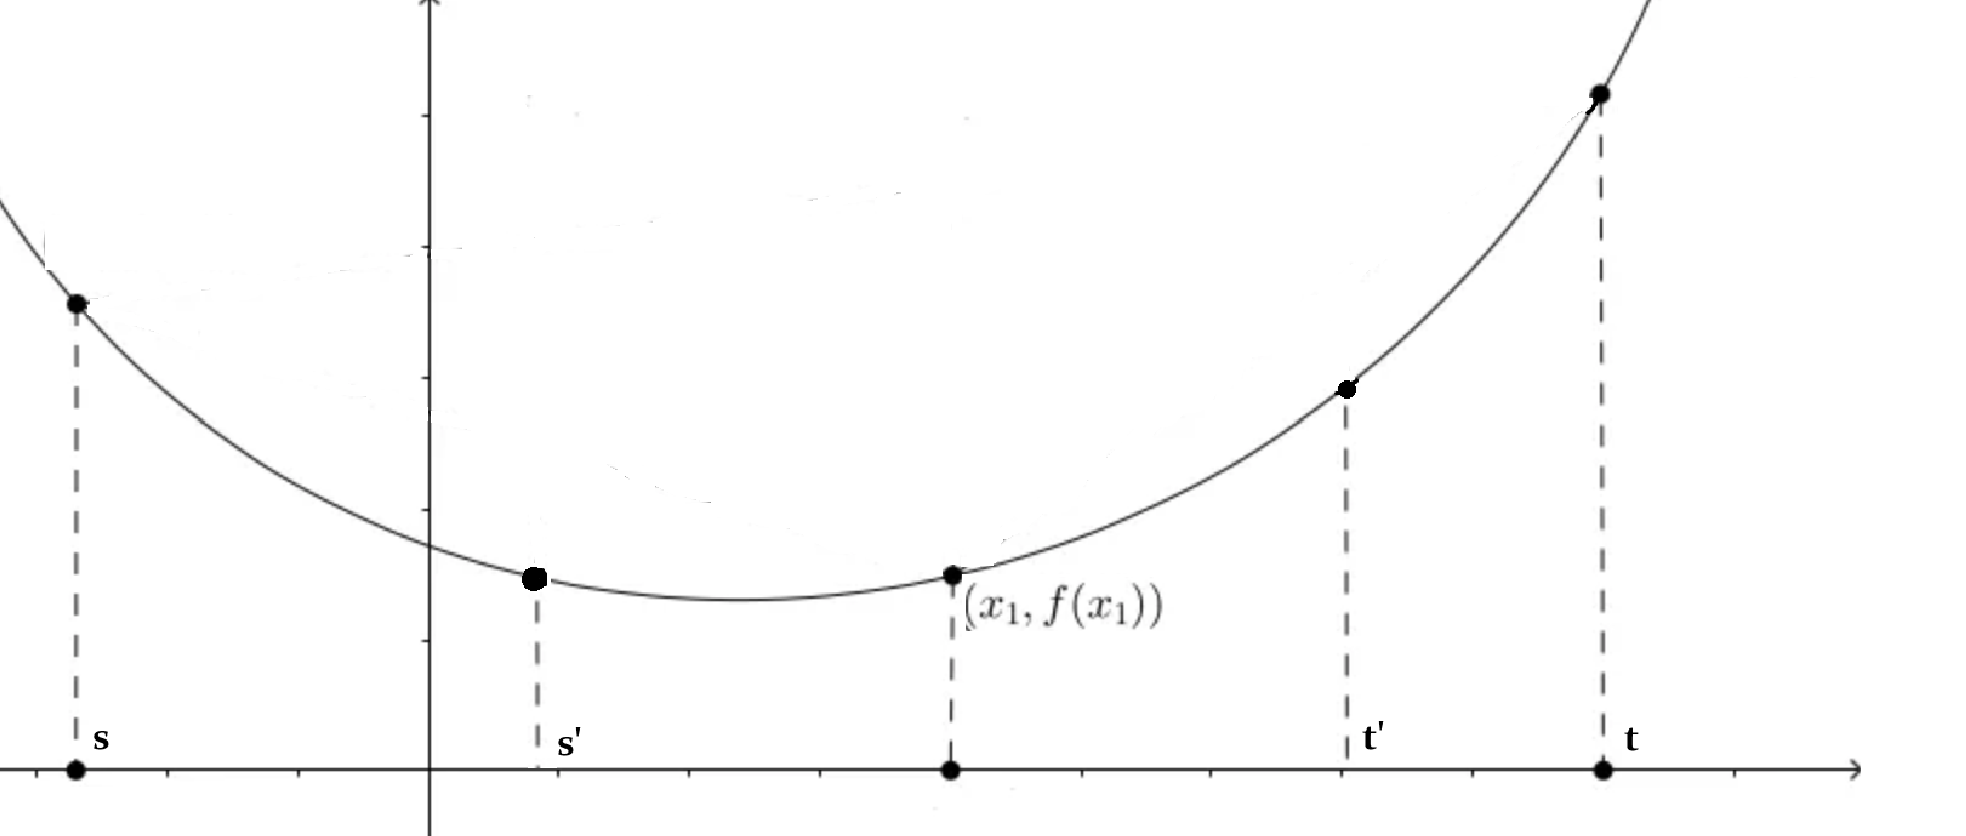
\includegraphics[width = 15cm]{assets/integral_1.png}
\end{center}

Заметим, что первая функция ограничена сверху второй, а вторая ограничена снизу первой. Откуда существуют  $f'_-(x_1), f'_+(x_1)$. Теперь применим теорему о предельном переходе в неравенствах и получим, что $f'_-(x_1)\leq f'_+(x_1)$.

Теперь докажем вторую часть.\\
Возьму $t$ на отрезке $(x_1,x_2)$. Посмотрю на  $\cfrac{f(t)-f(x_1)}{t-x_1}$ и $\cfrac{f(t)-f(x_2)}{t-x_2}$

Заметим, что исходя из этого, тк монотонно возрастает и ограниченна снизу и сверху (по тем же соображениям, что и до этого)
$$\exists  \lim\limits_{t \rightarrow x_1 + 0}\cfrac{f(t)-f(x_1)}{t-x_1} = f'_+(x_1)$$ и тк $\cfrac{f(t)-f(x_1)}{t-x_1}\leq\cfrac{f(x_2)-f(x_1)}{x_2-x_1}$ по лемме о трех хордах, то выполнено второе неравенство.
$$\exists  \lim\limits_{t \rightarrow x_2 - 0}\cfrac{f(t)-f(x_2)}{t-x_2} = f'_-(x_2)$$ и тк $ \cfrac{f(x_2)-f(x_1)}{x_2-x_1}\leq \cfrac{f(t)-f(x_2)}{t-x_2}$ по лемме о трех хордах, то выполнено третье неравенство.

\hfill Q.E.D.

\textbf{Следствие 1.} $f$ - выпукла на $\langle a,b\rangle \Rightarrow f$ непр на $(a,b)$.

\textbf{Следствие 2.} $f$ - выпукла на $\langle a,b\rangle \Rightarrow f$ не дифф. на $(a,b)$ в не более чем счетном множестве (множество точек разрыва НБЧС). Это верно, исходя из того, что значения правосторонних пределов и левосторонних растут (теорема об одностор дифф-ти вып. функции). и берем рациональное число на таком интеравле.

todo: добавить рисунок выпуклая вниз, выпуклая вверх

\thmm{Теорема (выпуклость в терминах касательных)}

$f$ - дифф. на $\langle a,b \rangle$. Тогда

$f$ - вып. вниз $\Leftrightarrow$ График $f$ лежит не ниже любой касательной:
$$\forall x_0,x \in \langle a,b\rangle: f(x) \geq f(x_0) + f'(x_0)(x-x_0)$$
\textbf{Доказательство:}

Докажем в правую сторону. Возьму $x>x_0$, тогда по предыдущей теореме: $f'(x_0)\leq \cfrac{f(x)-f(x_0)}{x-x_0}$. Домножу и победил. Аналогично $x<x_0$.

Докажем в левую сторону. Возьмем 3 точки, $x_1<x_0<x_3$:
$$f(x_3)\geq f(x_0)+f'(x_0)(x_3-x_0),\quad f(x_1)\geq f(x_0)+f'(x_0)(x_1-x_0)$$
$f'(x_0)\leq \cfrac{f(x_3)-f(x_0)}{x_3-x_0}$ и $ \cfrac{f(x_1)-f(x_0)}{x_1-x_0} \leq f'(x_0)$, тогда  по лемме о трех хордах $f$ выпукло.

\hfill Q.E.D.


\deff{def:} Дано множество $A$ выпуклое в $R^2$. Прямая $L$ называется \deff{опорной} к $A$ в точке $x_0$, если $L$ проходит через $x_0$ и множество $A$ лежит в одной полуплоскости (замкнутой).

\thmm{Теорема (дифф. критерий выпуклости)}

1) $f$ - дифф на $(a,b)$, непр на $\langle a,b \rangle$. Тогда $f$ - выпукло на $\langle a,b\rangle \Leftrightarrow f'$ возрастает на $(a,b)$.

2) $f$ непр на $\langle a,b \rangle$, $f$ - дважды дифф на $(a,b)$. Тогда $f$ - вып. $\Leftrightarrow f''\geq 0$ на $(a,b)$.

\textbf{Доказательство:}

1) $\Rightarrow$ очевидно из теоремы об односторонней дифф-ти.\\
$\Leftarrow$ Проверим утверждение леммы о трех хордах. 

$\cfrac{f(x_2)-f(x_1)}{x_2-x_1}= f'(c_1) $ по теореме Лагранжа.
$\cfrac{f(x_2)-f(x_2)}{x_3-x_2}= f'(c_2) $ по теореме Лагранжа.

Так как $c_1 < c_2$, а $f'$ возрастает, то нужное неравенство выполняется.

2) $f$ - выпуклое $\Leftrightarrow$ $f'$ возрастает $\Leftrightarrow$ $(f')'\geq 0 $

\hfill Q.E.D.
\pagebreak


\subsection{Правило Лопиталя.}

\thmm{Лемма (об ускоренной сходимости)}

Пусть даны $f,g: D \in R \rightarrow R$, $a$ - предельная точка $D$ в $\overline{\mathbb{R}}$

Пусть $\exists U(a), f,g \neq 0$ в $U(a)\cap D$ -  выколотой.

$\lim\limits_{x\rightarrow a}f(x) = 0, \lim\limits_{x\rightarrow a}g(x) = 0$. Тогда:
$$\forall (x_n): x_n \rightarrow a, x_n \in D, x_n \neq a,\exists (y_n): y_n \rightarrow a, y_n \in D, y_n \neq a: \lim\limits_{k \rightarrow \infty} \cfrac{f(y_k)}{g(x_k)}<\cfrac{1}{k}\text{ и}\lim\limits_{k \rightarrow \infty} \cfrac{g(y_k)}{g(x_k)}<\cfrac{1}{k}$$
\textbf{Доказательство:}

Давайте будем выбирать такие $y_k$, что:
$$\left|\cfrac{f(y_k)}{g(x_k)}\right|< \cfrac{1}{k} \text{ и }\left|\cfrac{g(y_k)}{g(x_k)}\right|< \cfrac{1}{k}$$

Очевидно, что мы сможем выбрать такие $y_k$. А из этого уже следует то, что нам надо.

\hfill Q.E.D.

\textbf{Замечание:} утверждение верно, если $\lim\limits_{x\rightarrow a}f(x) = +\infty, \lim\limits_{x\rightarrow a}g(x) = +\infty$

\thmm{Теорема(пр. Лопиталя)}

$f,g: (a,b) \rightarrow\mathbb{R}$, дифф $g'\neq 0$ на $(a,b)$

$\cfrac{f'(x)}{g'(x)} \xrightarrow{x \rightarrow a+0} A \in \overline{\mathbb{R}}$. Пусть $\lim\limits_{x\rightarrow a+0}\cfrac{f(x)}{g(x)}$ - неопределенность $\left(\cfrac{0}{0}, \cfrac{\infty}{\infty}\right)$

Тогда: $\lim\limits_{x\rightarrow a+0}\cfrac{f(x)}{g(x)}=\lim\limits_{x\rightarrow a+0} \cfrac{f'(x)}{g'(x)}$

\textbf{Доказательство:} 

Замечание о корректности: тк $g'\neq 0$, то $g$ - строго положительно или отрицательно в какой-то окрестности $a$.

По Гейне. Возьму $(x_n): x_n \rightarrow a,x_n\neq a$. Берем $y_n$ из Лопиталя. 

Теорема Коши: $\cfrac{f(x_k)-f(y_k)}{g(x_k)-g(y_k)} = \cfrac{f'(\xi_k)}{g'(\xi_k)}$, где $\xi_k \in (x_k, y_k)$.
$$\cfrac{f(x_k)}{g(x_k)} = \cfrac{f(y_k)}{g(x_k)} + \cfrac{f'(\xi_k)}{g'(\xi_k)}\left(1 - \cfrac{g(y_k)}{g(x_k)}\right)$$
    
Посмотрим, куда это стремится. Справа это стремится к $A$. Значит и слева должна.

\hfill Q.E.D.

\textbf{Пример неаналитической функции:}

\deff{Неаналитическая} - та, которую нельзя представить в виде разложение тейлора для бесконечности.

\textbf{Пример:}

$f(x) = \begin{cases}
    e^\frac{-1}{x}, x>0\\
    0,x\leq 0
\end{cases}$

$\forall x: \exists f^{(k)}(0) = 0$. Если разложить ее в нуле, то она будет эквивалентна нулевой


$a_{n+1}-a_n$ - аналог производной.

\thmm{Теорема (Штольца)}

$x_n,y_n$ - вещ. последовательности, $x_n \rightarrow 0 , y_n \rightarrow 0$. $y_n$ монотонный, начиная с какого-то места

Пусть $\lim\limits_{n\rightarrow \infty} \cfrac{x_{n+1}-x_n}{y_{n+1}-y_n} =  a\in \overline{\mathbb{R}}\cup \{0\}^*$. Тогда: $\exists \lim\limits_{n \rightarrow\infty}\cfrac{x_n}{y_n} = a$.

\textbf{Доказательство:}

1) $a>0, a \in \mathbb{R}$

$\forall a>\varepsilon>0:\exists N_1: \forall N>N_1: a-\varepsilon < \cfrac{x_{N+1}-x_N}{y_{N+1}-y_N} <a+\varepsilon$

Зафиксирую $N$. Возьму $n>N$ и напишу дроби $\cfrac{x_{N+1}-x_N}{y_{N+1}-y_N}$, $\cfrac{x_{N+2}-x_{N+1}}{y_{N+2}-y_{N+1}}$,\ldots, $\cfrac{x_{n}-x_{n-1}}{y_{n}-y_{n-1}}$.

Заметим интересный факт, что (для положит. дробей) $\cfrac{p}{q}<\cfrac{r}{s} \Rightarrow \cfrac{p}{q}<\cfrac{p+r}{q+s}<\cfrac{r}{s} $. Поэтому, если мы сложим, все вышесказанные дроби так, как показано, то они будут между $a-\varepsilon$ и $a+\varepsilon$. А вышесказанные дроби положит, потому что у нас начиная с какого-то места монотонен $y$ и $a>0$. Поэтому:
$$a-\varepsilon<\cfrac{x_n-x_N}{y_n-y_N}<a+\varepsilon$$
Что я получил? Устремим $n \rightarrow \infty$ и получим по условию, что $a-\varepsilon\leq\cfrac{x_N}{y_N}\leq a + \varepsilon$

2) $a = +\infty$. Аналогично, только смотрим на предел с одной стороны

3) $a = [-\infty, 0 )$, поменяем у $y_n: = -y_n$, тогда все стало положительным = счастье.

4) $a = 0$. Считаем, что $x_n, y_n$ монотонны (строго) с какого-то момента. Тогда дробь $\cfrac{x_{n+1}-x_n}{y_{n+1}-y_n} \rightarrow 0 $ с какого-то момента. Тогда  $\cfrac{y_{n+1}-y_n}{x_{n+1}-x_n} \rightarrow +\infty $, вернемся к пункту 1 и выиграем.

\hfill Q.E.D.

\textbf{Замечание.} Для неопределенности вида $+\infty,+\infty$ теорема верно (обе посл. монотонны). (Загадка)

\thmm{Теорема (Гаусса)}

Хотим доказать сумму $1 + 2 + \ldots + n = \cfrac{n(n+1)}{2}$.

\textbf{Доказательство:}

1) $x_n = 1 + 2 + \ldots + n$, Хочу найти $y_n$ такую, что
$\lim\limits_{n\rightarrow \infty} \cfrac{x_n}{y_n} = 1$. О чем нам говорит теорема Штольца? Что если $y$ будет таким, что $\lim\limits_{n\rightarrow \infty} \cfrac{x_{n}-x_{n-1}}{y_{n}-y_{n-1}} = 1$, то такой $y_n$ нам подходит

$y_n = n^2$ не подходит, $y_n = \cfrac{n^2}{2}$ подходит и дает в пределе 1. 
Мы доказали, что $1+2+3 +\ldots + n $ эквивалетно $n^2$. Но это еще не то, что нам надо

2) $x_n = 1+2+\ldots + n -\cfrac{n^2}{2}$, хотим опять по теореме Штольца найти чему это эквивалентно. $\lim \cfrac{x_n-x_{n-1}}{y_n-y_{n-1}} = \lim \cfrac{\frac{1}{2}}{y_n-y_{n-1}}=1$. О, возьму $y_n = \cfrac{n}{2}$. И все хорошо.

$1 + 2 + \ldots + n = \cfrac{n^2}{2} + \cfrac{n}{2} + o(n)$. Пока это тупик.

\hfill Q.E.D.

\textbf{Доказательство 2:}

$f(x) = x + x^2 + x^3 +\ldots + x^n$.

$f'(x) = 1 + 2x + 3x^2 + \ldots +x^n$

$xf'(x) = x + \ldots + nx^n  = (x\cfrac{d}{dx})f(x)$

$(x\cfrac{d}{dx})^Nf(x) = 1^Nx +2^Nx^2 +\ldots +n^Nx^n $

Заметим, что $f(x) = \cfrac{x^{n+1}-1}{x-1}-1$. Хочу посчитать значение функции в единице:
$$\left((x\cfrac{d}{dx})^Nf(x)\right)(1) =\left((x\cfrac{d}{dx})^N \left(\cfrac{x^{n+1}-1}{x-1}\right)\right)(1)$$
Заметим, что после $N$ раз дифференцирования знаменатель будет $(x-1)^{N+1}$. Но я хочу посчитать значение функции в точке $1$. Мы не можем так сделать, но заметим, что наша функция непрерывна, откуда мы знаем, что у нее есть предел  в этой точке. Применим $n+1$ раз правило Лопиталя идеологически??????? 

\textbf{Замечание от Славы. }Да именно такое говорит Константин Петрович на лекции в связи  с чем этот конспект хочется забросить и мне хочется выброситься в окно.  Так что со всех респект и уважение, что я сижу и разбираю.

Так что же тут подразумевал Константин Петрович? У нас  знаменатель будет $(x-1)^{N+1}$. Но значение функции в точке $1$ у нас есть. 

Из непрерывности мы знаем, что $(1^Nx +2^Nx^2 +\ldots +n^Nx^n)(1) = \lim\limits_{x \rightarrow 1} (1^Nx +2^Nx^2 +\ldots +n^Nx^n)$. И та наша формула, которую мы свернули с помощью геом. прогрессии ведет себя точно так же в окрестностях единицы. Также на самом деле числитель этой функции просто имеет множитель $(x-1)^{N+1}$. Поэтому мы можем думать, что мы ищем $\lim\limits_{x\rightarrow1} \cfrac{(x-1)^{N+1}\cdot h(x)}{(x-1)^{N+1}}$. Поэтому применим ${N+1}$ раз правило Лопиталя и знаменатель пропадет. Что мы получили? Мы получим, что теперь мы ищем предел по какой-то другой(непрерывной (тк многочлен)) функции при $x\rightarrow 1$. Значит, что мы можем просто посчитать значение в точке $1    $. Это то, что Константи Петрович назвал идеологически применить правило Лопиталя. То есть надо умножить нашу дробь на знаменатель $N$ раз ее продифференцировать и поделить на производную $N$-ой степени знаменателя:
$$= \cfrac{1}{(N+1)!}(\cfrac{d}{dx})^N\left((x-1)^{N+1}\left((x\cfrac{d}{dx})^N \left(\cfrac{x^{n+1}-1}{x-1}\right)\right)\right)$$
Дальше подставляете $N=1$ и все, ищите значение этой фигни в точке 1 и ваша жизнь прекрасна.

\hfill Q.E.D.







\pagebreak

\subsection{Определенный интеграл.}


\deff{def:} \deff{Фигура} - это ограниченное подмножество в $R^2$. $\varepsilon$ - множество всех возможных фигур.

$\sigma: \varepsilon \rightarrow [0,+\infty)$ ---  назовем \deff{площадью}, если:
\begin{enumerate}
    \item Аддитивно: $A_1,A_2 \in \varepsilon, A_1\cap A_2 = \emptyset, \sigma(A_1\cup A_2) = \sigma(A_1)+\sigma(A_2)$
\item Нормировка: $\sigma ([a,b]\times[c,d]) = (b-a)(d-c)$.
\end{enumerate}

\textbf{Замечание.} Площади существуют.

\textbf{Замечание.} \begin{enumerate}
    \item Она обладает монотонностью по включению: $A \subset B, \sigma(A) \leq \sigma(B)$, так как: $B = A + (B \setminus A) \Rightarrow \sigma(B) = \sigma(A) + \sigma(B \setminus A)$.
    \item $\sigma(\text{вертик отрезок})=0$, так как его площадь всегда меньше окружающего его прямоугольника с шириной и высотой $= \forall \varepsilon > 0$.
\end{enumerate}

\deff{def:}  $\sigma:\varepsilon\rightarrow [0,+\infty)$ --- \deff{ослабленная площадь}, если выполнено:
\begin{enumerate}
    \item монотонна.
    \item нормирована.
    \item ослабленная аддитивность: Есть $E \in \varepsilon: l $ - вертик. прямая $L^-$ - левая полуплоскость, $L^{+}$ - правая полуплоскость (замкнутая полуплоскость), тогда  $E_1 = E\cap L^-, E_2 = E \cap L^+: \sigma(E)=\sigma(E_1)+\sigma(E_2)$
\end{enumerate}

Пример осл. площади:
\begin{enumerate}
    \item $\sigma(A) = \inf (\sum \sigma(P_k), \text{где $A = \bigcup\limits_{\text{конеч}}P^k, \text{где $P_k$ - прямоугольник}$})$ 
    \item $\sigma(A) = \inf (\sum \sigma(P_k), \text{где} A = \bigcup P^k, \text{где $P_k$ - прямоугольник})$
\end{enumerate}

todo: написать отличие.

\deff{def:} \deff{Срезка} - $f:\langle a,b\rangle \rightarrow \mathbb{R} $.
\begin{enumerate}
    \item \uline{положительная} --- $f^+ = \max(f,0)$
    \item \uline{отрицательная} --- $f^- = \max(-f,0)$
\end{enumerate}

todo: вставить рисунок

\deff{def:} $f:[a,b] \rightarrow \mathbb{R}, f\geq 0$ ПГ $(f,[a,b]) = \{(x,y): x\in [a,b], y \in [0,f(x)]\}$.

\deff{def:} $f: [a,b] \rightarrow \mathbb{R}$, $f$ - непр., $\sigma $- осл. адд площадь, тогда \deff{определенный интегралом} $f$ по отрезку $[a,b]$ назовем: $$\dint\limits_{a}^b f =\dint\limits_{a}^b f(x) dx =\sigma(\text{ПГ($f^+$,$[a,b]$)})-\sigma(\text{ПГ($f^-$,$[a,b]$)})$$

\textbf{Простейшие свойства:}
\begin{enumerate}
    \item Если $f \ge 0$ на $[a, b]$, тогда $\integral{a}{b}f \ge 0$
    \item Если $f = c$ (константа), тогда $\integral{a}{b}c = c \cdot (a - b)$
    \item $\integral{a}{b}(-f) = -\integral{a}{b}f$
    \item $\integral{a}{a}f = 0$
\end{enumerate}

\textbf{Свойства интеграла:}
\begin{enumerate}
    \item Аддитивность по промежутку: $\forall c \in [a,b]:\dint\limits_{a}^b =\dint\limits_{a}^c + \dint\limits_{c}^b $
    \item Монотонность: $f\leq g$ - непр., то $\dint\limits_{a}^b f(x)\leq \dint\limits_{a}^b g(x)$. 

    Говорят: Проинтегрируем неравенство $f\leq g$, на отрезке $[a,b]$.

    \item $(b-a)\min_{[a,b]} f \leq\integral{a}{b}f\leq (b-a)\max_{[a,b]}f$

    Делается с помощью монотонности и интегрирования $\min_{[a,b]}f\leq f\leq\max_{[a,b]}$А

    \item $\left|\integral{a}{b}f(x)dx\right|\leq \integral{a}{b}|f(x)|dx$

    Проинтегрируем $-|f|\leq f\leq |f|$ и получим то, что хотим.

    \item \thmm{Теорема о среднем}

    Функция $f \in C([a,b])$. Тогда $\exists c \in [a,b]$, что:
    $$\integral{a}{b}f = f(c)(b-a)$$
    \textbf{Доказательство:} 
    
    $a=b$ - скучно. Если $a\neq b$, напишем неравенство п.3:
    $$\min f\leq \cfrac{1}{b-a}\integral{a}{b}f\leq \max f$$ А мы знаем, что функция непрерывна, тогда по теореме о промежуточном значении:
    
    $$\exists \, c  = \cfrac{1}{b-a}\integral{a}{b}f$$. 
    
    \hfill Q.E.D.
\end{enumerate}

\deff{Интеграл с переменным верхним пределом} -  $\Phi:[a,b] \rightarrow R: \Phi(x)= \integral{a}{x}f$

\deff{Интеграл с переменным нижним пределом} -  $\psi:[a,b] \rightarrow R: \psi(x)= \integral{x}{b}f$

для $f\in C([a,b])$.

\thmm{Теорема (Барроу)}

В усл. определений. Доказать, что $\Phi$ дифф на $[a,b]$, $\Phi'(x)=f(x)$.

\textbf{Доказательство:}

$y> x: \lim\limits_{y \rightarrow x+0} \cfrac{\Phi(y)-\Phi(x)}{y-x} = \lim\limits_{y \rightarrow x+0} \cfrac{\int_a^y f - \int_a^x f}{y-x} =\lim\limits_{y \rightarrow x+0} \cfrac{1}{y-x} \integral{x}{y}f =\lim_{y\rightarrow x+0} f(c)$, \\
где $c$ лежит между $x,y$ из теоремы о среднем.

Получим, что правосторонняя производна равна $f(x)$. Аналогично про левостороннюю. Откуда производная это $f(x)$.

 \hfill Q.E.D.
 
\textbf{Замечание} Мы построили первообразную для функции $f$.

\thmm{Теорема (формула Ньютона-Лейбница)}

$f\in C([a,b])$, $F$ - первообразная $f$ на $[a,b]$. Тогда

$\integral{a}{b}f(x)dx = F(b)-F(a) = F(x)\big|^b_a$

\textbf{Доказательство:}

$F = \Phi + c$, по теореме 2. Поэтому сделаем некоторые преобразования:
$$\integral{a}{b}f(x)dx = \Phi(b)= \Phi(b)-\Phi(a) = (F(b)-c)-(F(a)-c)=F(b)-F(a)$$
 \hfill Q.E.D.

 \textbf{Следствие:} Этот определенный интеграл не зависит от выбора $\sigma$. 
 
 \textbf{Замечание:} Откажемся от соглашения $a\leq b$ и введем для $d<c:$
 $$\integral{c}{d}= - \integral{d}{c} = F(d) - F(c)$$
 \thmm{Микротеорема (Линейность интеграла)}

 Для $f,g \in C([a,b])$, $\alpha,\beta \in \mathbb{R}$, выполнено:
$$\integral{a}{b}\alpha f+ \beta g = \alpha \integral{a}{b}f + \beta\integral{a}{b}g$$
\textbf{Доказательство:}

$(\alpha F+\beta G)\big|^b_a = \alpha F\big|^b_a + \beta F|^b_a$ из линейности неопредел. интеграла.
 \hfill Q.E.D.

 \thmm{Теорема (Интегрирование по частям)}

 $f,g \in C^1([a,b])$. Тогда $\integral{a}{b}fg' = fg\big|_a^b-\integral{a}{b}f'g$

 \textbf{Доказательство:}

Из теоремы  о свойствах неопределенного интеграла:
$$fg = \text{првобр} (fg'+f'g) \Rightarrow \integral{a}{b}(fg' + f'g) = fg\big|_{a}^b$$
 \hfill Q.E.D.
 
 \thmm{Теорема (о замене переменных)}

$f \in C(\langle a,b\rangle), \,\, \varphi\langle\alpha, \beta\rangle \rightarrow \langle a, b \rangle, \,\, \varphi \in C^1, \,\, [p,q] \subset \langle \alpha,\beta\rangle$. Тогда:
$$\integral{p}{q}f(\varphi(t))\varphi'(t)dt = \integral{\varphi(p)}{\varphi(q)}f(x)dx$$
\textbf{Доказательство:}

$F$ - первообразная $f$, тогда $F(\varphi(t))$ - первообразная $f(\varphi(t))\varphi'(t)$ и все получается.
 
 \hfill Q.E.D.

1:09 мат анализ кохась лекция 2. Я ничего не понял про нижние два замечания


 \textbf{Замечание.} Может показаться, что множество $\varphi([p,q])$ шире $[\varphi(p),\varphi(q)]$. 

 \textbf{Замечание.} Может быть, что $\varphi(p) > \varphi(q)$

$I_f$ - среднее значение $f$  на $[a,b]$  $\cfrac{1}{b-a}\integral{a}{b}f$
 
 \thmm{Теорема (Неравенство Чебышёва)}

 $f,g \in C([a,b])$ обе возрастают. Тогда $I_f \cdot I_g \leq I_{fg}$, то есть
$$\integral{a}{b}f \cdot \integral{a}{b}g\leq (b-a)\integral{a}{b}fg$$
\textbf{Доказательство:}

Тк функции возрастают, то $\forall x,y \in [a,b]: (f(x)-f(y))(g(x) - g(y))\geq 0$.
$$f(x)g(x)-f(y)g(x)-f(x)g(y) + f(y)g(y) \geq 0$$ 
Давайте зафиксируем $y$ и проинтегрируем по $x$ и поделю на $b-a$. Получу:
$$I_{fg} - f(y) I_g - I_f g(y) + f(y)g(y)\geq 0 $$
Давайте зафиксируем $x$ и проинтегрируем по $y$ и поделю на $b-a$. Получу:
$$I_{fg}-I_fI_g -I_gI_f + I_{fg} \geq 0$$
\hfill Q.E.D.

\textbf{Пример (Ш. Эрмит)} \\
Пусть мы хотим посчитать $H_n = \cfrac{1}{n!}\integral{-\frac{\pi}{2}}{\frac{\pi}{2}} \left(\cfrac{\pi^2}{4}-t^2\right)^n \cos t dt$\\
$\integral{a}{b}fg' = fg\Big|^a_b - \integral{a}{b}f'g$. Воспользуюсь этим в дальнейших рассуждениях\\
$H_n =\left [ \begin{array}{l}
    f = \left(\cfrac{\pi^2}{4}-t^2\right)^n\\  
     g = \cos t 
\end{array}\right] =\left(\cfrac{\pi^2}{4}-t^2\right)^n \sin t\Bigg|^{\pi/2}_{\pi/2} + \cfrac{2}{(n-1)!}\integral{-\pi/2}{\pi/2}t(\cfrac{\pi^2}{4}-t^2)^{n-1}\sin t dt $

я не хочу это писать 1:30 2 лекция

$H_n = (4n-2)H_{n-1} - \pi^2H_{n-2} = P(\pi^2)$ - многочлен, от $\pi^2$, где $\deg P\leq n$.

\thmm{Теорема (Пи иррационально)}

$\pi$ - иррационально. Проверим, что $\pi^2$ иррационально. 

\textbf{Доказательство:}

Пусть $\pi^2 = \cfrac{p}{q}$. Тогда $q^nH_n=\cfrac{q^n}{n!}\integral{-\pi/2}{\pi/2}\left(\cfrac{\pi^2}{4}-t^2\right)^n \cos t \,\, dt = q^n P(\pi^2)$ - целое число. А слева неотрицательная функция.

$0<q^nH_n \leq \cfrac{q^n}{n!}4^n\pi=\cfrac{(4q)^n}{n!}\pi\rightarrow 0$, но с другой стороны, оно должно быть целым. Противоречие.

\hfill Q.E.D.

\deff{def:} $f:[a.b] \rightarrow \mathbb{R}$ \deff{кусочно-непрерывной.}

$\exists A \ = \{x_1,\ldots,x_n\} \subset [a,b]$. Такая функция будет непрерывны на $[a,b]$, кроме этих точек, а в них происходят скачки.


\deff{def:} $F:[a,b] \rightarrow \mathbb{R}$ - \deff{почти первообразная} функции f, если:

$F$ - непр и $\exists A = \{x_1,\ldots,x_n\} \subset[a,b]$.
$\forall x \in [a,b] \textbackslash A: \exists F'(x) = f(x)$ и $\forall x \in A: \exists F'_+(x),F'_-(x)$


$f$ - кусочно-непрерывно на $[a,b]$. $x_0 = a, x_n = b$. Положим $\integral{a}{b} = \sum\limits_{i=1}^{n+1}\integral{x_{i-1}}{x_i}f\Big|_{[x_{i-1},x_i]}$

\textbf{Утверждение.} Если $f$ - кусочно - непрерывна тогда: $\integral{a}{b}f=F(b)-F(a)$.

Утверждение очевидно по определению.

\textbf{Следствие:} Все теоремы, использующие в доказательство только формулу Ньютона-Лейбница у нас уже доказаны!

\textbf{Пример (Неравенство Чебышева для сумм)}

$a_1\leq \ldots \leq a_n, b_1\leq \ldots \leq b_n$.

Тогда $\displaystyle\left(\cfrac{1}{n} \sum\limits_{i=1}^na_ib_i\right)\geq \left( \cfrac{1}{n}\sum a_i\right)\left(\cfrac{1}{n}\sum b_i\right)$

\textbf{Доказательство:}
\begin{center}
   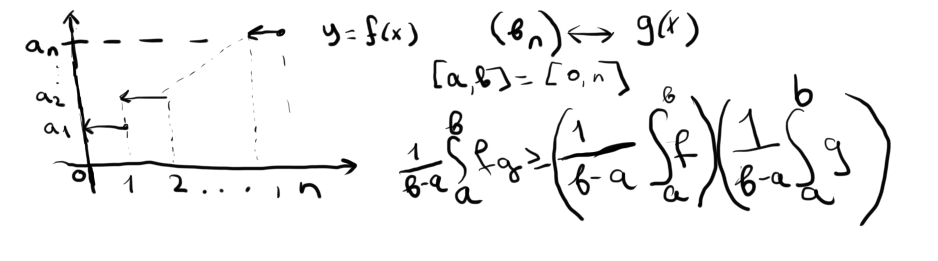
\includegraphics[width = 19 cm]{assets/integral_2.png}
\end{center}
Возьмем доску Константина Петровича для лучшего понимания. Давайте возьмем две функции $f(x)$, $g(x)$, как показано на рисунке. Вспомним, что у нас есть неравенство Чебышева, которое записано на правой стороне доски. Тогда очевидно подстановкой в него наших $f(x),g(x)$ и $a=0,b=n$, мы получим нужное неравенство.
\hfill Q.E.D.

\pagebreak
\subsection{Приложение к определенным интегралам.}

Введем некоторые обозначения:

$\Segm ([a,b])$ - множество всевозможных отрезков, лежащих в $[a,b]$

$\varPhi: \Segm([a,b]) \rightarrow \mathbb{R}$ - \deff{функция для промежутка}.

Введем \deff{аддитивные функции для промежутка}:
$$\forall [p,q] \in \Segm[a,b]: \forall c \in (p,q): \varPhi([p,c]) + \varPhi(c,q)= \varPhi([p,q])$$

\deff{def:} $f: \langle a,b \rangle \rightarrow \mathbb{R}$, $\varPhi: \Segm(\langle a,b \rangle) \rightarrow \mathbb{R}$ - а.ф.п:

$f$ - \deff{плотность} $\varPhi$: $\forall \Delta \in \Segm (\langle a,b\rangle):$$inf_{\Delta} f \cdot len(\Delta)\leq \varPhi(\Delta)\leq sup_{\Delta} f \cdot len(\Delta)$

\thmm{Теорема(о вычисл. а.ф.п.по ее плотности)}

Дана плотность
$f:\langle a,b\rangle \rightarrow \mathbb{R}$, $\varPhi: \Segm(\langle a,b\rangle)$ - а.ф.п., $f$ - непр.

Тогда $\forall \Delta \in \Segm(\langle a,b\rangle) $, $\varPhi(\Delta) = \integral{\Delta}{}f$

\textbf{Доказательство:}

Н.У.О. считаем, что $\Delta = [a,b]$. Тогда возьмем $F(x)$, такую что:
$$F(x) = \left[ 
      \begin{gathered} 
        0, x=a \\ 
        \varPhi([a,x]), x \in (a,b) \\ 
      \end{gathered} 
\right.$$
Проверим, что $F$ - первообразная f:

$F'_{+}(x) = \cfrac{F(x+h)-F(h)}{h} = \cfrac{\varPhi([a, x +h])-\Phi([a,x])}{h} = \cfrac{\varPhi(x,x+h)}{h}\in [\min f, \max f]$ на промежутке $x+x_0$ из ее плотности  

Получили, что правосторонняя производная $f$ и левостороняя производные существуют.

\hfill Q.E.D.



\uline{\textbf{Пример: Площадь криволинейного сектора.} }

$[a,b] \subset [0,2\pi)$

$\rho:[a,b]\rightarrow \mathbb{R}, \rho>0$

$\varphi \in [a,b] \rightarrow (\varphi,\rho(\varphi))$

Введем определение: \deff{Сектор} $[\alpha,\beta] = \{(\varphi,r)\subset R^2: \varphi\in[\alpha,b], 0\leq r\leq p(\varphi)\}$

$\varPhi: \Delta = \sigma(\text{Сектора}) $, $\Delta \in \Segm([a,b])$


\thmm{Теорема (Площадь криволинейного сектора).}  

В указанных условия, а так же $\rho: [a,b] \rightarrow \mathbb{R}, \rho>0$ и непрерывна. $[\alpha,\beta]\in \Segm([a,b])$. Тогда: $$\varPhi([\alpha,\beta]) = \cfrac{1}{2}\integral{\alpha}{\beta}\rho^2(\varphi) \, d\varphi$$
\textbf{Доказательство:}

Если мы докажем, что $\frac{1}{2}\rho^2(\varphi)$ - плотность $\varPhi$, тогда по предыдущей теореме, мы получим, что данная формула будет верна. Будем опрделять определение плотности.

$\Delta = [\alpha,\beta]$, откуда Сектор$[\alpha,\beta]\subset$ Криволинейного вектора($O, \max \rho, [\alpha,\beta]$).

Криволинейный вектор в в данном случае подразумевает сектор окружности, нарисованный на чертеже. Так же на нем вы видите серым - Сектор$[\alpha,\beta]$.

\begin{center}
   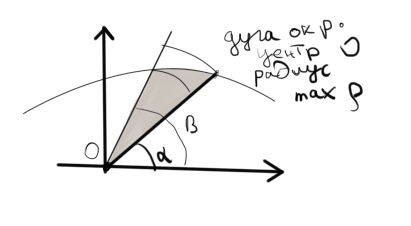
\includegraphics[width = 10 cm]{assets/integral_3.png}
\end{center}

Как мы знаем из геометрии: площадь сектора окружности = $\cfrac{\alpha}{2}R^2$.

Откуда из монотонности площади:
$$\varPhi([\alpha, \beta])\leq \sigma(\text{Крив. вектор}) = \cfrac{1}{2} (\beta-\alpha) (\max\limits_{[a,b]}\rho)^2$$
Аналогично можно оценить нижним сектором. То есть:
$$\cfrac{1}{2} (\beta-\alpha) (\min\limits_{[a,b]}\rho)^2\leq\varPhi([\alpha, \beta])\leq \cfrac{1}{2} (\beta-\alpha) (\max\limits_{[a,b]}\rho)^2$$
Откуда это и правда плотность, поэтому верно.

\hfill Q.E.D.

\textbf{Кохась: хочу эксперимент}

$\sigma (\text{ПГ($f, [a,b]$)}) = \integral{a}{b}f\, dx$, где $f \geq 0, f$ - непрерывно.
$\gamma(t) =  \left (\begin{gathered}
    x = x(t)\\
    y(x) = y(t)
\end{gathered}\right)$, $\gamma:[p,q] \rightarrow R^2$.
\begin{center}
   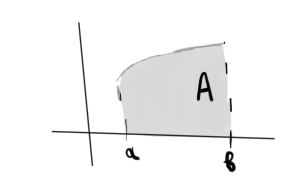
\includegraphics[width = 7 cm]{assets/integral_4.png}
\end{center}
\textbf{Замечание от Славы}: вообще $x(t)$ должно монотонно возрастать, иначе странные загагулины будут давать одну и ту же площадь, но КПК про это ничего не сказал.

Причем $\gamma$ -  гладкое изоображение (дифференцируема столько раз сколько надо).

Получилась какая-то кривая (как на рисуночке сверху), и я хочу смотреть подграфики такой кривой. Тогда:
$$\sigma A = \integral{a}{b}"y(x)"dx = \left[\begin{gathered}
    x = x(t)\\
    y = y(t)
\end{gathered}\right] = \integral{p}{q}y(t) x'(t) dt$$
Теперь мы умеем вычислять интегралы не только в декартовых координатах.

todo: вставить 2 формулы 1.50

\textbf{Пример:}

$\begin{cases}
    x(t) = r(t-\sin(t)), r\in R\\
    y(t) = r(1-\cos(t)), t \in[0,2\pi]
\end{cases}$ - путь, который описывается данной формулой - \deff{циклоид}.

Фиксируем точку в нуле и катим окружность по нашему полю. Мы знаем, что $x$ монотоннен
\begin{center}
   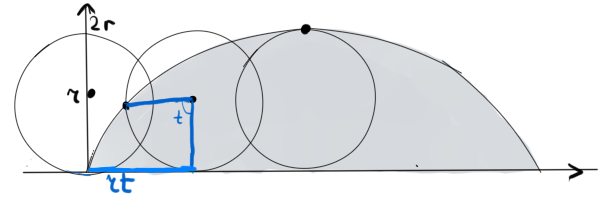
\includegraphics[width = 13 cm]{assets/integral_5.png}
\end{center}
И теперь я хочу найти площадь серого подграфика:

$S  = \integral{0}{2\pi r}y(x)dx  = \left [ \begin{gathered}
    x(t) = r(t-\sin t) \\
    y(t) = r(1-\cos t)
\end{gathered}\right] = \integral{0}{2\pi}r^2(1-\cos t)^2 dt = r^2\integral{0}{2\pi}(1-\cos t)^2 = 3 \pi r^2$


\textbf{Пример (Изопериметрическое неравентсво.)}

$G \subset \mathbb{R}^2$ - выпукло, замкнуто, ограниченно. 

Пусть $diam(G) = \sup\limits_{a,b\in G} (\rho(a,b))$ - диаметр. $diam(G) = d$. Тогда: $\sigma(G)\leq \cfrac{\pi}{4}d^2$

todo: тут во-первых скипнут рисунок, во-вторых я не осознал 2:20

$\rho(\varphi) = \max (r: (\varphi,r)_{max} \in G)$ -  непрерывна.

Упражнение: доказать непрерывность (возможно спросят на экзамене)

$\overline{\varphi} = \varphi + \cfrac{\pi}{2}$

$$\sigma(G)= \frac{1}{2}\integral{-\frac{\pi}{2}}{\frac{\pi}{2}}\rho^2(\varphi)\,d\varphi = \frac{1}{2}\left(\integral{0}{\frac{\pi}{2}} + \integral{\frac{-\pi}{2}}{0}\right) = \frac{1}{2}\integral{\frac{-\pi}{2}}{0}\rho^2(\varphi)\, d \varphi  + \cfrac{1}{2}\integral{0}{\frac{\pi}{2}}\rho^2\left(\overline{\varphi}-\cfrac{\pi}{2}\right)\,
d\overline{\varphi}=$$

$$=\frac{1}{2}\integral{\frac{\pi}{2}}{0}\rho^2(\varphi) + \rho^2(\varphi - \frac{\pi}{2}) d\varphi = \cfrac{1}{2}\integral{0}{\frac{\pi}{2}}"AB^2" d\varphi \leq \cfrac{1}{2}\integral{0}{\frac{\pi}{2}}d^2 d\varphi = \frac{d^2\pi}{4}$$

\thmm{Теорема (обобщ. теорема о плотности)}

$\varPhi: Segm(\langle a,b\rangle) \rightarrow \mathbb{R}$ - а.ф.п. $f: \langle a,b \rangle \rightarrow \mathbb{R}$ - непрерывно.

Пусть $\forall\Delta \in Segm(\langle a,b \rangle)$ заданы $m_\Delta, M_{\Delta} $ - функции от сегмента:

\begin{enumerate}
    \item $m_\Delta\cdot l(\Delta) \leq \varPhi(\Delta) \leq M_{\Delta} \cdot l(\Delta)$
    \item $\forall x  \in \Delta: m_{\Delta}\leq f(x)\leq M_{\Delta}$
    \item $\forall$ фикс. $x\in \langle a,b \rangle$, $M_{\Delta}-m_{\Delta}\rightarrow 0$, при $l(\Delta)\rightarrow 0 $ и $x\in \Delta$ 
\end{enumerate}
Тогда $f$ - плотность $\varPhi$. 

\textbf{Доказательство:}

Н.у.о мы работаем на $[a,b]$.  $F(x) = \begin{cases}
    \varPhi([a,x]), x>a\\
    0,x =a
\end{cases}$

Напишем то, что нам дает условие в конкретной точке $x$:
$$m_{\Delta}\leq\cfrac{F(x+h)-F(x)}{h}\leq M_{\Delta}\text{, где }\Delta = [x,x+h], h>0$$
$$m_\Delta \leq f(x) \leq M_{\Delta}$$
Вычтем из одного другое:
$$\left|\cfrac{F(x+h)-F(x)}{h } -f(x)\right|\leq M_{\Delta}-m_{\Delta}$$
Устремим $h$ к нулю и получим, что $M_{\Delta}-m_{\Delta} \rightarrow 0$. Откуда $\left|\cfrac{F(x+h)-F(x)}{h } -f(x)\right|\rightarrow 0 $, а это $f(x) = F_{+}'(x)$. Аналогично $f(x) = F'_i(x) $.

\hfill Q.E.D.

1.48 - 4 лекция - кохась рассказывает интересную историю про отрубленные пальцы

\textbf{Пример (Объем вращения фигур)}

\begin{center}
   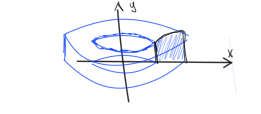
\includegraphics[width = 10 cm]{assets/integral-v-figure.png}
\end{center}

$a>0,b>0, f>0$. Вращаем ПГ$(f[a,b])$ вокруг оси $Oy$. Получается вот что-то такое(см рисунок). Хочу найти объем этой фигуры 

$\varPhi([a,b]) = Vol(\{(x,y,z): a^2\leq x^2 + y^2 \leq b^2, 0\leq z \leq f(\sqrt{x^2+y^2})\})$. Тогда выполнено:
$$\varPhi([a,b]) = 2\pi \integral{a}{b}xf(x)dx$$
\textbf{Доказательство:}

$A_1$ - прямоугольник, такой что его высота $ = \min\limits_{(a,b)}f$. $A_1 = [a,b] \times [0,\min f]$

$Vol A_1 = \pi b^2 \min f - \pi a^2 \min f$

$A_2$ - прямоугольник, такой что его высота $ = \max\limits_{(a,b)}f$. $A_2 = [a,b] \times [0,\max f]$

$Vol A_2 = \pi b^2 \max f - \pi a^2 \max f$.

$\forall \Delta$ положим $m_{\Delta} = \pi \min_{\Delta
}f \cdot \min(2x) $, $M_{\Delta} = \pi \max_{\Delta} f \cdot \max 2x$, $x\in \Delta$ 

Тогда: как мы только что доказали: $$\varPhi(\Delta)\leq Vol(A_2(\Delta)) = \pi \max f \cdot (\overline{b}+\overline{a})(\overline{b}-\overline{a})\leq M_{\Delta}(\overline{b}-\overline{a})\leq M_{\Delta}l(\Delta)$$
Выше в формуле подразумеваются текущие $\overline{a},\overline{b}$ для $\Delta$. Аналогично для $m_{\Delta}$.

При $x \in \Delta: m_{\Delta}\leq \pi f(x)2x\leq M_{\Delta}$ - очевидно.

Фиксируем $x: M_{\Delta}-m_{\Delta}\rightarrow 0 $ при $\Delta \rightarrow0$ - очевидно. Откуда выполнено условие теоремы о плотности а это то, что нам и требовалось.

\hfill Q.E.D.

\textbf{Пути:}

$\gamma :[a,b] \rightarrow \mathbb{R}^m$. То есть $t\rightarrow (\gamma_1(t),\gamma_2(t),\ldots,\gamma_m(t)) = \gamma(t)$. Мы обычно думаем, что они непрерывны

$\lim\limits_{\tau \rightarrow 0} \cfrac{\gamma(t + \tau )-\gamma(t)}{\tau}$ - интересно как меняется.

$\gamma'(t) = (\gamma_1'(t),\gamma_2'(t),\ldots,\gamma_m'(t))$ - \deff{вектор скорости}.

\deff{Носитель пути} - траектория пути.

\deff{def:} Функция $l$, заданная на множестве гладких путей (непрерывны, дифференцируемы) называется длиной пути, если выполняются следующие условия:

\begin{enumerate}
    \item $l\geq 0$
    \item аддитивна: $\forall [a,b]$, $\forall \gamma:[a,b]\rightarrow\mathbb{R}^m$ для любого $c\in [a,b]: l(\gamma) = l(\gamma\Big|_{[a,c]}) + l(\gamma\Big|_{[c,b]})$
    \item $\gamma, \overline{\gamma}$ --- два пути. $C_{\gamma},C_{\overline{\gamma}}$ --- носители пути.
    
    Если $\exists T: C_{\gamma} \rightarrow C_{\overline{\gamma}}$ --- сжатие ($\forall M,N:\rho(T(M), T(N))\leq \rho(M,N)$), то $l(\overline{\gamma})\leq l(\gamma)$
    \item $\gamma$ - линейный путь, то $l(\gamma) = \rho(A,B)$, где $A$ - начало, $B$ - конец.
\end{enumerate}

А такая штука вообще существует? 
    
\textbf{Замечание:} Из свойства 3 следует, что длина хорды меньше длины дуги.

\textbf{Замечание:} При растяжении длина пути растет.

\textbf{Замечание:} Длина пути не меняется при движениях пространства $R^m$ (очевидно из свойства 3).

\thmm{Теорема:}

$\gamma: [a,b] \rightarrow \mathbb{R}^m$ - $C^1$ - непрерывно дифференцируемо. Тогда $l(\gamma) = \integral{a}{b}||\gamma'(t)||dt$.

\textbf{Доказательство:}

Считаем $\gamma$ - инъективный.

$[p,q]\in Segm[a,b]: \varPhi([p,q]) = l(\gamma\Big|_{[p,q]})$. Проверим $||\gamma'(t)||$ - плотность $\varPhi$.

$\Delta:\forall i = 1,\ldots,m: m_i(\Delta) = \min_{\delta} |\gamma'_{i}(t)|$, $M_i(\Delta) = \max|\gamma_i'(t)|$.

Возьму $m_{\Delta} = \sqrt{\sum\limits_{i=1}^m m_i^2(\Delta)}$, $M_{\Delta} = \sqrt{\sum\limits_{i=1}^m M_i^2(\Delta)}$. Проверяем 1, 2, 3 из обобщенной теоремы о плотности. 2 и 3 очевидно выполнены. 

Проверим 1: $m_{\Delta} l(\Delta) \leq \varPhi(\Delta)\leq M_\Delta l(\Delta)$. Завожу $\overline{\gamma}:\Delta \rightarrow R^m$ - линейный путь: $\gamma(t) = (M_1(\Delta)t,M_2(\Delta)t,\ldots,M_m(\Delta)t)$. Строю $T: C_{\gamma} \rightarrow C_{\overline{\gamma}}$, такое, что $\gamma(t) \rightarrow \overline{\gamma}(t)$. Проверим, что это растяжение. Давайте считать расстояние. $\rho(\gamma(t_0),\gamma(t_1)) = \sqrt{\sum\limits_{i=1}(\gamma_i(t_0)-\gamma_i(t_1))^2}$. По теореме Лагранжа: $$\sqrt{\sum\limits_{i=1}(\gamma_i(t_0)-\gamma_i(t_1))^2} =\sqrt{ \sum \gamma_i'(\tau_i)(t_0-t_1)^2} =\sqrt{\sum \gamma_i'(\tau_i)}|t_0-t_1| \leq M_{[t_0,t_1]}|t_0-t_1|$$
$$\leq M_{\Delta}|t_0-t_1| = \rho(T(\gamma(t_0)),T(\gamma(t_1)) =\rho(\overline{\gamma}(t_0),\overline{\gamma}(t_1))$$
Откуда выполнен пункт один и выполнена обобщенная теорема о плотности.


\hfill Q.E.D.

\textbf{Примеры:}
\begin{enumerate}
    \item В $\mathbb{R}^2:\gamma(t) = (x(t),y(t))$ - обычные декартовы.

    $$l = \integral{a}{b}\sqrt{x'(t)^2+y'(t)^2} dt$$
    \item $\mathbb{R}^2$, полярные координаты $r(t)$,$\varphi(t)$
    $$l = \integral{a}{b} \sqrt{((r(t) \cos \varphi(t))')^2+((r(t) \sin\varphi(t))')^2} = \integral{a}{b} \sqrt{r(t)^2+r'(t)^2}dt$$
    \item Длина графика $x(t) =t, y(t) = f(t)$. 
    $$l = \integral{a}{b}\sqrt{1 + y'(x)^2}dx$$
\end{enumerate}

Вернемся к вопросу существованию такой штуки.

\textbf{Существование длины пути} - Супремум длин вписанных ломаных. Разбиваю отрезок на $n$ кусочков и считаю сумму длины ломанных: $a=x_1<x_2<\ldots<x_n =b$

Теперь будем рассматривать пути в $\mathbb{R}^1$.

$l(\gamma) = \sup (\sum\limits\gamma(t_k)-\gamma(t_{k-1}) | a = t_0<t_1<\ldots<t_n=b)$.

\textbf{Замечание:} $\gamma \in C^1:$ $l(\gamma) = \integral{a}{b}|\gamma'(t)|dt$.

\textbf{Замечание:} Пусть $f$ - любая из $[a,b] \rightarrow \mathbb{R}$. Тогда \deff{вариация функции} на $[a,b]$: $$\Var_a^b f = \sup (\sum\limits_{k=1}^n |f(t_k)-f(t_{k-1})|)$$
Пример:
$f(x) = \begin{cases}
    1,x \in \Q \\
    0, x \in \R, x\not \in \Q 
\end{cases}$, $\Var_{a}^b f = +\infty$

Если для $f$ выполнено: $\Var_a^b f < + \infty$, то она называется \deff{ограниченной} вариации.

\textbf{Экскурсия в зоопарк.}

\deff{Кривая Пеано} - это путь в $\R^2$, такой, что я сначала разбиваю отрезок $[0,1]$ на 4 равных части так, что отображение первой части отрезка находится в части 1(см рисунок), второй части отрезка в части 2 и так далее. Потом повторяю то же самое в каждом квадратике. Потом повторяю то же самое в каждом квадратике квадратика и так далее. Изображение внизу описывает это построение поэтапно.

\begin{center}
   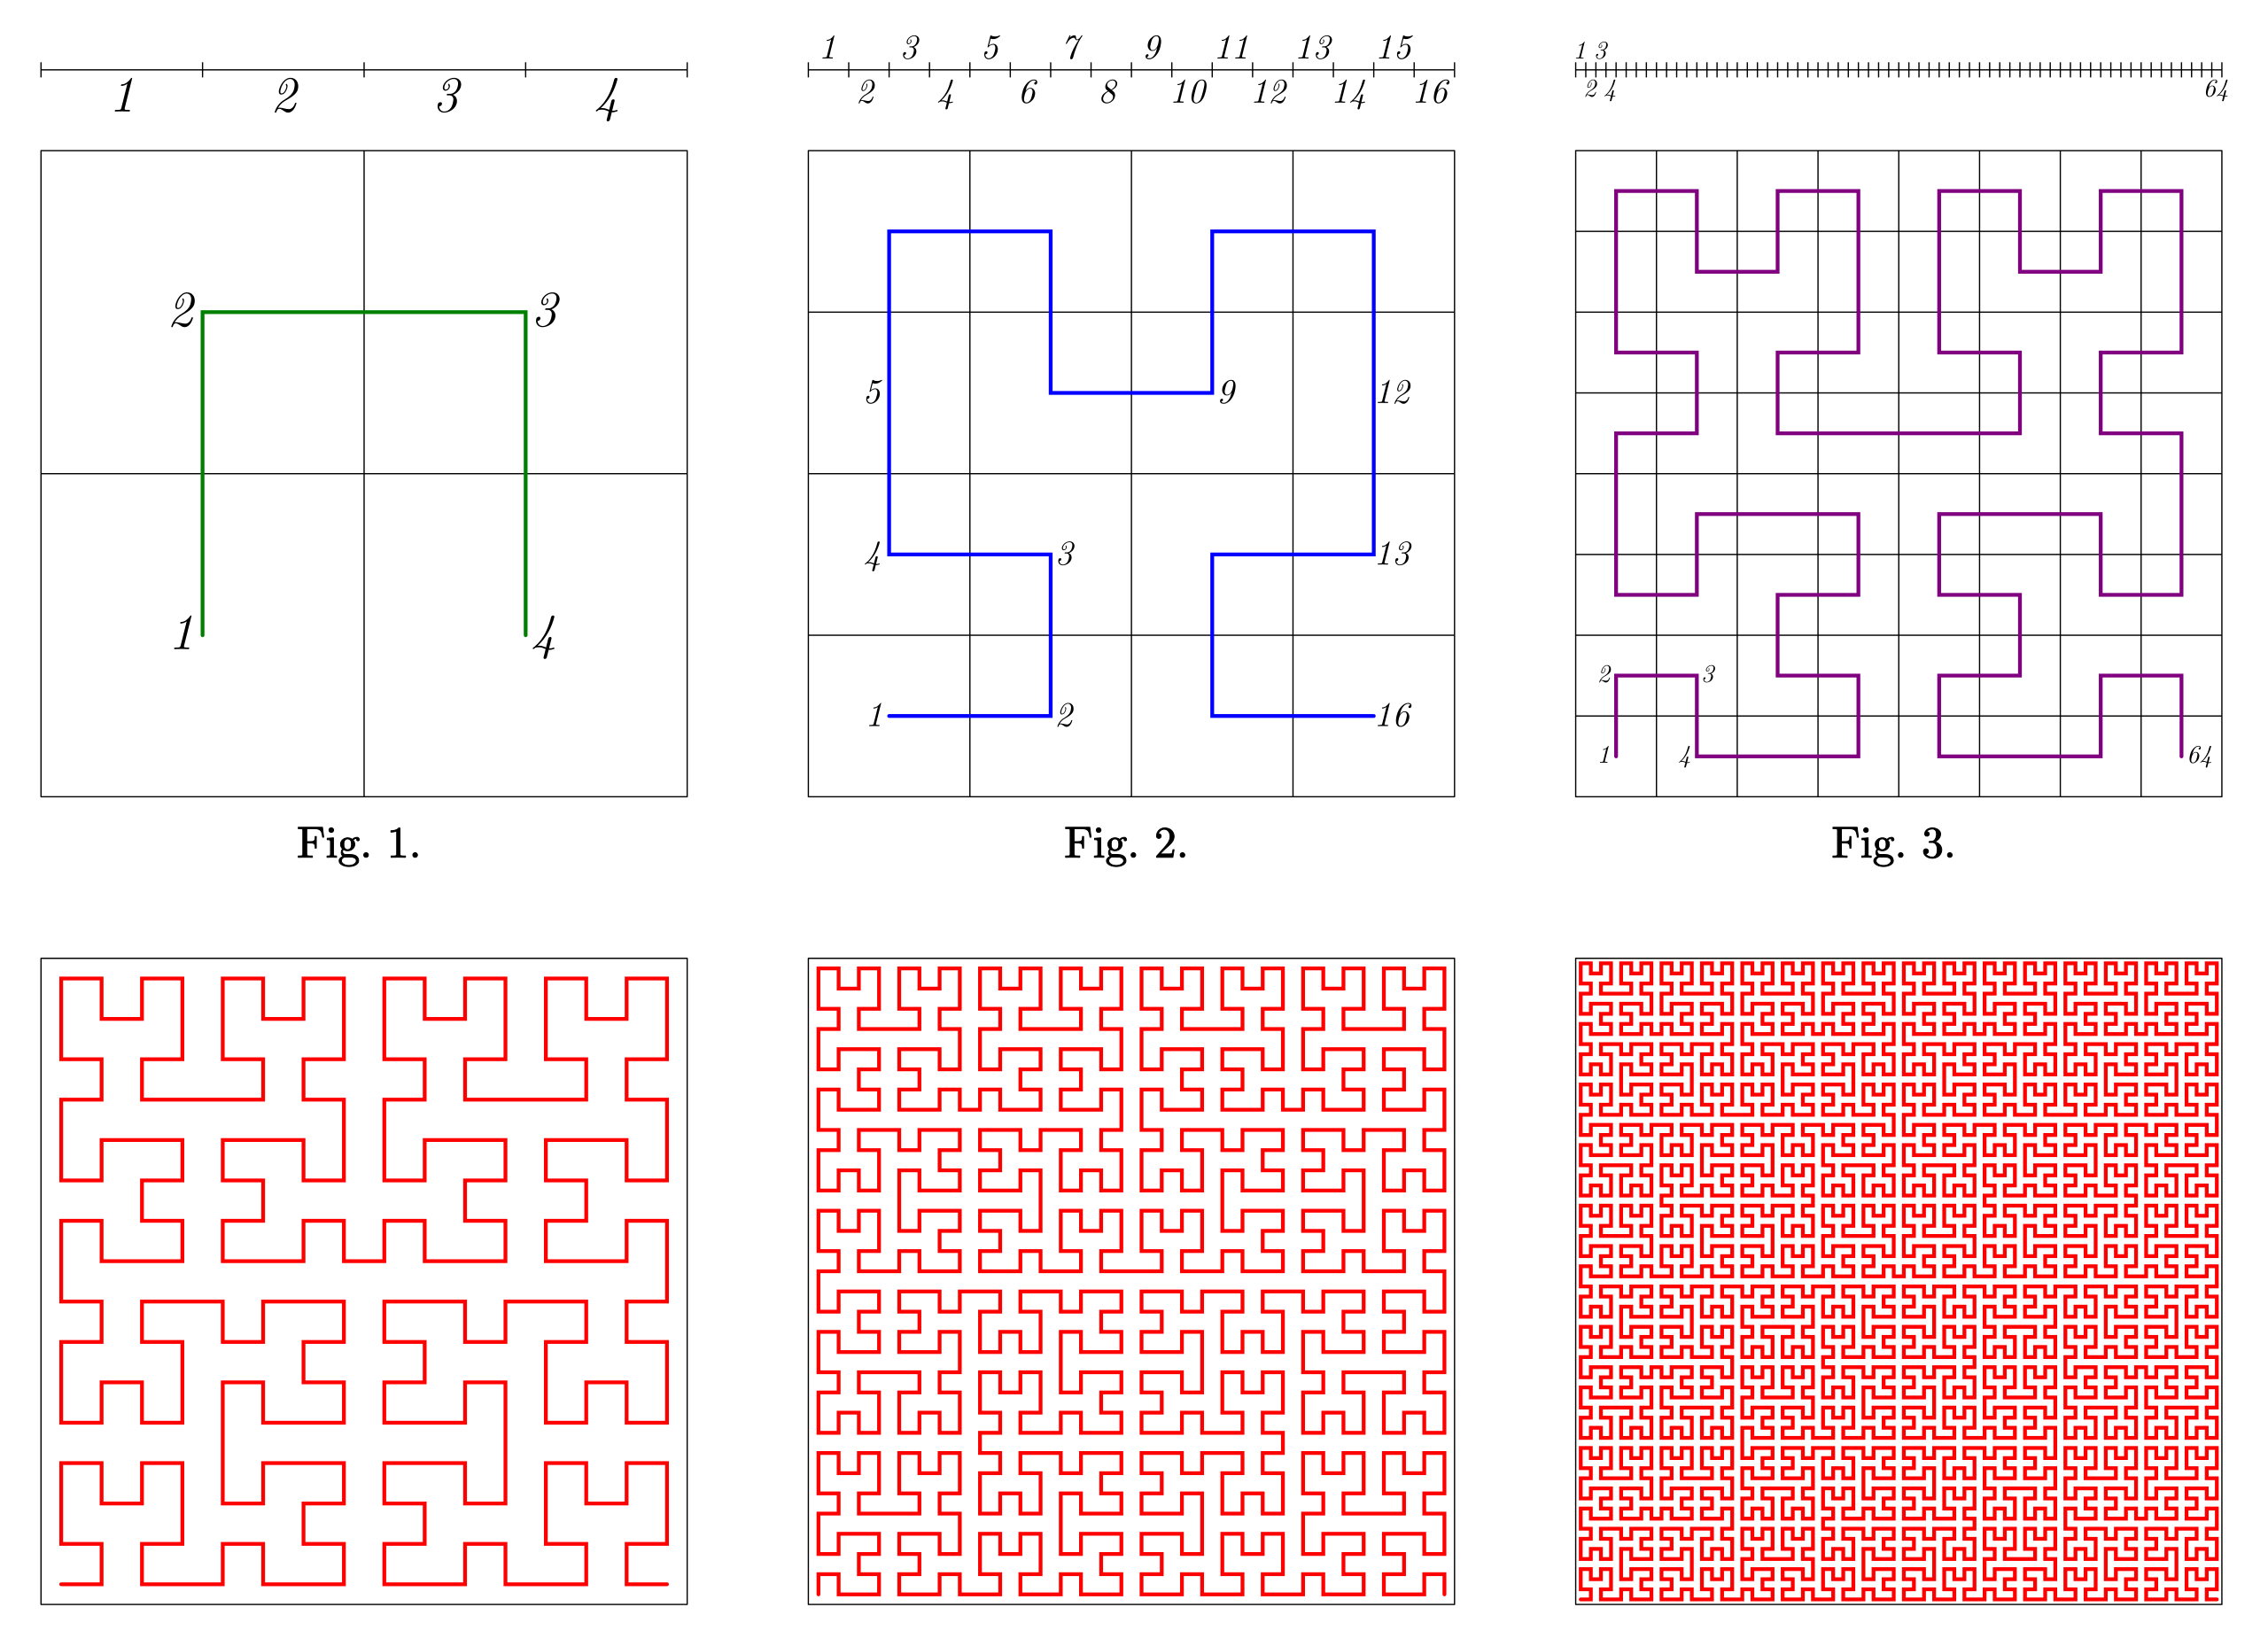
\includegraphics[width = 15 cm]{assets/integral_hilbert_curve.svg.png}
\end{center}

Заметим, что у нас биекция между $\R$ и в $\R^2$. 

\newpage
\subsection{Верхний и нижний пределы последовательностей}

\deff{def:} $(x_n)$ - вещ. последовательность $L\in \mathbb{R}$ - \deff{частичный предел} $x_n: \exists (n_k):n_1<n_2<\ldots: \lim\limits_{n\rightarrow \infty} x_{n_k}=L$.

\deff{def:} $x_n$ - вещ. последовательность. Рассмотрим $y_n = \sup (x_n, x_{n+1},\ldots),z_n = \inf(x_n,x_{n+1},\ldots)$. $y_n$ - \deff{верхне огибающая}, $z_n$ - \deff{нижне огибающая}. 

$y_n$ - не возрастает, $z_n$ - не убывает. $\forall n: z_n\leq x_n \leq y_n$

Если изменить конечное число членов последовательности, то $y_n,z_n$ изменятся конечное число раз.

\deff{Верхний предел последовательности}--- $\overline{\lim\limits_{n\rightarrow \infty}}x_n=\lim y_n \in \overline{R}$

\deff{Нижний предел последовательности}--- $\underline{\lim\limits_{n\rightarrow \infty}}x_n=\lim y_n \in \overline{R}$

\thmm{Теорема (о свойствах верхнего и нижнего предела)}

$(x_n), (\overline{x_n})$ --- произвольные вещ последовательности

\begin{enumerate}
    \item $\underline{\lim}x_n \leq \overline{\lim }x_n$
    \item Если $\forall n : x_n \leq \overline{x_n}$, то $\overline{\lim} x_n\leq \overline{\lim} \overline{x_n}$ и $\underline{\lim} x_n\leq \underline{\lim} \overline{x_n}$
    
    \textbf{Замечание от Славы:} На самом деле здесь можно сказать, что $\exists N$ начиная с которого выполнено $x_n \leq \overline{x_n}$, но КПК почему-то решил так ввести это свойство.

    \item $\forall \lambda \in\mathbb{R}, \lambda\geq 0$. Тогда $\overline{\lim}\lambda x_n = \lambda \overline{\lim} x_n$ и $\underline{\lim}\lambda x_n = \lambda \underline{\lim} x_n$. (Считаем $0 \cdot \infty = 0$)
    \item $\overline{\lim}(-x_n)= - \underline{\lim}x_n$
    \item $\overline{\lim }(x_n + \overline{x}_n) \leq \overline{\lim }  {x}_n + \overline{\lim }\overline{x}_n $
    \item Пусть $t_n \rightarrow l \in \R$. Тогда $\overline{\lim}(x_n + t_n) = \overline{\lim} (x_n) + l $ и $\underline{\lim}(x_n + t_n) = \underline{\lim} (x_n) + l $
    \item $t_m \rightarrow l>0 (l\in \R)$. Тогда $\overline{\lim} (t_nx_n) =l  \overline{\lim} (x_n)$ и  $\underline{\lim} (t_nx_n) =l  \underline{\lim} (x_n)$
\end{enumerate}

\textbf{Доказательство:}
\begin{enumerate}
    \item т.к. $\forall n: z_n\leq x_n \leq y_n$, то используем теорему о предельном переходе и получим то, что нам надо.
    \item Используем теорему о предельном переходе и получим то, что нам надо.
    \item Очевидно из свойств предела.
    \item Очевидно из свойств супремума.
    \item $\sup(x_n + \overline{x_n}, \ldots)\leq \sup(x_n,\ldots) + \sup(\overline{x}_n)$ - первое значение в паре не больше $\sup(x_n,\ldots)$, второе не больше $\sup(\overline{x}_n)$.
    \item $\forall \varepsilon >0: \exists N_0: \forall x > N_0: x_k+ l - \varepsilon < x_k + t_k < x_k + l + \varepsilon$ - верно из условия.

    Возьмем $N> N_0$ при $n\geq N$ выполнено, откуда перейдем к супремумам множеств:
    $$y_N + l - \varepsilon \leq \sup (x_N + t_N, x_{N+1} + t_{N+1},\ldots )\leq y_N + l + \varepsilon$$
    Устремлю $N$ к бесконечностти:
    $$\overline{\lim} y_n + l - \varepsilon \leq \lim \sup(...)\leq \overline{\lim} y_n + l + \varepsilon $$
    \item Аналогично прошлому пункту.
\end{enumerate}

\hfill Q.E.D.

\thmm{Теорема (техническое определение верхнего предела).}

$(x_n)$ - произвольная вещ. последовательность.

\begin{enumerate}
    \item $\overline{\lim}x_n = + \infty \Leftrightarrow x_n$ - не ограничено сверху
    \item $\overline{\lim}x_n = - \infty \Leftrightarrow x_n \rightarrow - \infty$.
    \item $\overline{\lim}x_n = l \Leftrightarrow$
    \begin{enumerate}
        \item $\forall \varepsilon >0: \exists :\forall n>N: x_n<l+\varepsilon$
        \item $\forall \varepsilon >0$ неравенство $l-\varepsilon\leq x_n$ выполнено для бесконечного множества $x$-ов
    \end{enumerate}
\end{enumerate}

\textbf{Доказательство:}

\begin{enumerate}
    \item Очевидно.
    \item $x_n\leq y_n$ Тогда по теореме о предельном переходе(или двух городовых) $x_n \rightarrow -\infty$. А в обратную сторону очевидно из определения предела.
    \item $\Rightarrow$ $\forall  \varepsilon: \exists N: \forall n> N: x_n\leq y_n < \varepsilon+l$ - пункт а доказан просто определением предела $y_n$.

    $\forall \varepsilon >0: \exists N:\forall n >  N: l-\varepsilon < y_n$. 
    
    Тогда по техническому описанию супремума $\exists k \geq n : l-\varepsilon < x_k \leq y_n$. Потом возьмите $n>k$ и так далее. Мы научились делать бесконечное кол-во таких $k$-шек, откуда пункт б доказан.
    
    $\Leftarrow$ $y_n$ - убывающая. Если мы имеем a, то $\forall \varepsilon>0: \exists N: \forall n > N: x_n < l + \varepsilon$. Из этого следует $y_n\leq l + \varepsilon$. И благодаря пункту б у нас выполнено техническое описание супремума то есть $y_n \rightarrow l$
\end{enumerate}

\hfill Q.E.D.

\thmm{Теорема}

$\exists \lim(x_n) = L \in \overline{\mathbb{R}} \Leftrightarrow \underline{\lim}x_n = \overline{\lim} x_n = L$.

\textbf{Доказательство:}

$L = + \infty$ - см прошлую теорему. Аналогично c $-\infty$.

$L\in \mathbb{R}$. В правую сторону очевидно из технического описания. В левую сторону: $z_n\leq x_n\leq y_n$ по теореме о двух городовых верно.

\hfill Q.E.D.


\thmm{Теорема о характеризации верхнего предела как частичного}

$(x_n)$ - вещ последовательность. Тогда:

\begin{enumerate}
    \item Если $l \in \overline{\mathbb{R}} - $ частичный предел $x_m$, то $\underline{\lim}x_n\leq l \leq \overline{\lim}x_n$
    \item $\exists n_k, m_k: x_{n_k}\rightarrow \overline{\lim} x_{n}, x_{m_k}\rightarrow \underline{\lim}x_n$
\end{enumerate}

\textbf{Доказательство:}

\begin{enumerate}
    \item $x_{n_k} \rightarrow l$: $z_{n_k}\leq x_{n_k}\leq y_{n_k}$. Устремим к $+\infty$ и получис то, что надо.
    \item Очевидно из технического описания супремума и техн. описания верхнего предела (будем выбирать все более и более близкие к l).
\end{enumerate}

\hfill Q.E.D.



\newpage
\subsection{Интегральные суммы.}

\deff{def:} $[a,b]$ \deff{дробление} отрезка $[a,b]$ (на $n$ частей):

$x_0 = a <x_1<x_2<\ldots <x_n=b$.

\deff{Ранг} дробления(мелкость) - $\max |x_k-x_{k-1}|$

\deff{Оснащение дробления} - $\{\xi_1,\ldots, \xi_n\}: \xi_i \in [x_{i-1},x_i]$

Пусть задана $f:[a,b] \rightarrow \R$. Тогда \deff{Риманова сумма}: $\sum\limits_{i=1}^n f(\xi_i)(x_i-x_{i-1})$.

\thmm{Теорема(об интеграле, как о пределе частичных сумм)}

$f\in C([a,b])$. Тогда $\forall \varepsilon >0: \exists \delta >0 : \forall$ дробления $(x_0,\ldots,x_m)$ ранга $< \delta$. Тогда $\forall$ оснащ.:
$$\left|\integral{a}{b}f(x)dx - \sum\limits_{i=1}^nf(\xi_i) (x_i-x_{i-1})\right|<\varepsilon$$
\textbf{Доказательство:}

Используем теорему Кантора о равномерной непрерывности: $$\forall \varepsilon> 0: \exists \delta >0: \forall x,\overline{x} \in [a,b]: |x-\overline{x}|<\delta: |f(x) - f(\overline{x})|<\varepsilon$$
$$\integral{a}{b}f(x)dx - \sum\limits_{i=1}^nf(\xi_i)(x_i-x_{i-1})= \sum\limits_{i=1}^n \integral{x_{i-1}}{x_i}f(x)dx - f(\xi_i)(x_i-x_{i-1}) = $$
$$=\sum\limits_{i=1}^n \integral{x_{i-1}}{x_i}f(x)dx - \integral{x_{i-1}}{x_i}f(\xi_i)dx  = \sum\limits_{i=1}^n \integral{x_{i-1}}{x_i}(f(x) - f(\xi_i))dx $$
Теперь возьму $\delta$ и $\epsilon$ из теоремы Кантора, возьму любое дробление ранга меньше $\delta$, получу, что $|x_i-\xi_i|<\delta$ и $|\xi_i- x_{i-1}|<\delta$. Откуда выполнено теорема Кантора и разность $|f(x)-f(\xi_i)|<\varepsilon$. Откуда:
$$\left|\integral{a}{b}f(x)dx - \sum\limits_{i=1}^nf(\xi_i) (x_i-x_{i-1})\right| \leq \sum\limits_{i=1}^n \integral{x_{i-1}}{x_i}|(f(x) - f(\xi_i))|dx\leq \sum\limits_{i=1}^n \integral{x_{i-1}}{x_i}\varepsilon dx = \varepsilon(b-a)$$
Откуда по теореме о бюрократном учете получим искомое.

\hfill Q.E.D.

$w(\delta) = \sup\limits_{t,x \in [a,b], |x-t|<\delta} |f(t) - f(x)|$ --- \deff{модуль непрерывности}.


\thmm{Теорема (об интегральной сумме центральных прямоугольников)}

$f \in C^2([a,b])$, $a = x_0<x_1<\ldots< x_n =b$, $\delta = max(x_i-x_{i-1}), \xi_i = \cfrac{(x_{i-1}+x_i)}{2}$.

Тогда:
$$\left|\sum\limits_{i=1}^m f(\xi_i)(x_i-x_{i-1}) - \integral{a}{b}f(x) dx\right|\leq \cfrac{\delta^2}{8}\integral{a}{b} |f''(x)|dx$$
\thmm{Теорема (формула трапеций)}

в тех же условиях:
$$\left|\sum\limits_{i=1}^n (\cfrac{f(x_i)+f(x_{i-1})}{2}(x_i-x_{i-1}))-\integral{a}{b}f(x) dx\right|\leq \cfrac{\delta^2}{8}\integral{a}{b} |f''(x)|dx$$
\textbf{Доказательство:}

$$\integral{x_{i-1}}{x_i}f(x)dx =\integral{x_{i-1}}{x_i}f(x)(x-\xi_i)'dx=f(x)(x-\xi_i)\Big|_{x_{i-1}}^{x_i} - \integral{x_{i-1}}{x_i}f(x) (x-\xi_i)dx =$$
$$= (f(x_i)+f(x_{i-1}))\cdot \cfrac{x_i-x_{i-1}}{2} + \cfrac{1}{2}\integral{x_{i-1}}{x_i}f'(x)((x-x_{i-1})(x_i-x))'dx = $$
$$=[\psi_i(x) = (x-x_{i-1})(x_i-x)]= ... +\cfrac{1}{2} f'(x)\psi_i(x) \Big|_{x_{i-1}}^{x_i} - \cfrac{1}{2}\integral{x_{i-1}}{x_i}f''(x) \psi_i(x)dx $$
Тогда:
$$\left |\sum \cfrac{f(x_i)-f(x_{i-1})}{2}(x_i-x_{i-1})-\integral{a}{b}f(x)dx \right| = \left| \sum\limits_{i=1}^n\cfrac{1}{2}\integral{x_{i-1}}{x_i}f''(x)\psi_i(x) dx\right|$$
Заметим, что $\psi(x)$, которая является функцией из частей $\psi_i(x)$ будет непрерывной, откуда я могу ее интегрировать и сделать замену на нее:
$$\left| \sum\limits_{i=1}^n\cfrac{1}{2}\integral{x_{i-1}}{x_i}f''(x)\psi(x) dx\right| = \left| \cfrac{1}{2}\integral{a}{b}f''(x)\psi_(x) dx\right|\leq \cfrac{1}{2}\integral{a}{b}\left|f''(x)\psi(x)\right|dx \leq \cfrac{\delta^2}{8}\integral{a}{b} |f''(x)|dx$$
\hfill Q.E.D.

\thmm{Формула Эйлера - Маклорена (простейшая)}

$f \in C^2([m,n])$, $m,n \in \mathbb{R}$. Тогда:

$\sum\limits_{i=m}^n f(i) - \cfrac{1}{2}f(m) - \cfrac{1}{2}f(n)= \integral{m}{n}{f(x)}{dx}+ \cfrac{1}{2}\integral{m}{n}f''(x)\{x\}(1-\{x\})dx$

\textbf{Доказательство:}

Очевидно :)

Это буквально прошлая теорема, просто надо очень долго пялится в формулу.  $\psi(x) = (1-\{x\})\{x\}$. Попяльтесь в формулу и тоже поймете.

\hfill Q.E.D.

\textbf{Примеры:}

$f(x) = x^p$ $(p> -1)$
$$1^p+2^p+\ldots + n^p= \integral{1}{n}x^pdx + \cfrac{1}{2}(n^p+1)+\cfrac{1}{2}\integral{1}{n}p(p-1)x^{p-2}\{x\}(1-\{x\}) =$$$$= \cfrac{n^{p+1}}{p+1}-\cfrac{1}{p+1}+\cfrac{n^p}{2}+\cfrac{1}{2} + O(\max(1,n^{p-1}) = \cfrac{n^{p+!}}{p+1} + \cfrac{n^p}{2} + O(max(1,n^{p-1}))$$
Торжественный момент, применим формулу для $p=1$:

$1 + 2 + \ldots + n = \cfrac{n^2}{2}+\cfrac{n}{2}+0$ --- Мы доказали теорему Гаусса.

Применим формулу для $p=-1$:

$1+ \cfrac{1}{2}+ \cfrac{1}{3}+ \ldots + \cfrac{1}{n} = \ln n + \cfrac{1}{2} + \cfrac{1}{2n}+\integral{1}{n}\cfrac{1}{x^3}\{x\}(1-\{x\})dx$

$1+\cfrac{1}{2}+\cfrac{1}{3}+\ldots +\cfrac{1}{n}= \ln n + \gamma + o(1)$. Причем $\gamma \in [\cfrac{1}{2},\cfrac{5}{8}]$ - \deff{Постоянная Эйлера}


\deff{Формула Валлиса}

$I_n = \integral{0}{\frac{\pi}{2}}\sin^nxdx = \begin{cases}
    \cfrac{(n-1)!!}{n!!}\cfrac{\pi}{2}, n - \text{четная}\\
    \cfrac{(n-1)!!}{n!!}, n - \text{неч}
\end{cases}$

КПК: Используйте формулу интегрирования по частям. Двойной факториал - одной четности

$x\in [0,\frac{\pi}{2}]$

$\sin^{2k+1} x\leq \sin^{2k}x\leq \sin^{2k-1}x$ - очевидное неравенство. Проинтегрируем по $0,\cfrac{\pi}{2}$, получим:
$$\cfrac{(2k)!!}{(2k+1)!!}\leq \cfrac{(2k-1)!!}{2k!!}\cdot \cfrac{\pi}{2}\leq \cfrac{(2k-2)!!}{(2k-1)!!}$$
$$\left(\cfrac{(2k)!!}{(2k-1)!!}\right)^2\cfrac{1}{2k+1} \leq \cfrac{\pi}{2}\leq \left(\cfrac{(2k)!!}{(2k-1)!!}\right)^2\cfrac{1}{2k}$$
Правая часть - левая часть $\left(\cfrac{(2k)!!}{(2k-1)!!}\right)^2(\cfrac{1}{2k}\cdot\cfrac{1}{2k+1})\leq \cfrac{\pi}{2}\cdot \cfrac{1}{2k} \rightarrow 0$

Получили, что левая и правые величины стремятся к $\frac{\pi}{2}$.

$\lim\limits_{k\rightarrow\infty}\left(\cfrac{(2k)!!}{(2k-1)!!}\right)^2\cfrac{1}{k} = \pi$ --- \deff{Формула Валлиса}

\thmm{Формула Стирлинга}

Воспользуемся формулой Эйлера - Маклорена для $f(x) = \ln x$:
$$\ln 1 + \ln 2 + \ldots + \ln n = \integral{1}{n}\ln x dx +\cfrac{\ln n }{2} - \cfrac{1}{2}\integral{1}{n}\cfrac{1}{x^2}\{x\}(1-\{x\})dx = $$
$$n\ln n - n + 1 +\cfrac{\ln n}{2} - \cfrac{1}{2}\integral{1}{n}\cfrac{1}{x^2}\{x\}(1-\{x\})dx = n \ln n - n +\cfrac{\ln 2}{2} +C_1 + o(1)$$
А давайте теперь возвем экспоненту от правой и левой части:
$$n! = e^{n\ln n}e^{-n}e^\frac{\ln n}{2} e^{C_i + o(1)}$$
Получили, что $n!\, \mytilde\, \cfrac{n^n}{e^n}\sqrt{n}\cdot c$, где $c = e^{C_1}$.

А теперь давайте сочетать и найдем эту $c$.

$(2k)!! = k!\cdot 2^k, (2k-1)!! = \cfrac{(2k)!}{k!\cdot2^k}$. С учетом этого воспользуемся формулой Валлиса:
$$\sqrt{\pi} = \lim\limits_{k\rightarrow\infty}\left(\cfrac{(2k)!!}{(2k-1)!!}\right)\cfrac{1}{\sqrt{k}}=\lim_{k\rightarrow \infty}\cfrac{2^{2k}(k!)^2}{(2k)!}\cfrac{1}{\sqrt{k}} = \lim_{k\rightarrow \infty} \cfrac{2^{2k}k^{2k}e^{-2k}k\cdot c^2}{(2k)^{2k}e^{-2k}\sqrt{2k}\cdot c}\cfrac{1}{\sqrt{k}} = \cfrac{c}{\sqrt{2}}$$
Откуда $c = \sqrt{2\pi}$

$n!\, \mytilde\, \cfrac{n^n}{e^n}\sqrt{n}\cdot \sqrt{2\pi}$ --- \deff{Формула Стирлинга}

\newpage 
\subsection{Несобственные интегралы.}

\deff{def:} \deff{Допустимая функция} на $[a,b): (-\infty<a<b\leq + \infty)$

$\forall A \in (a,b): f$ - кусочно непрерывная на $[a,A]$

\deff{def:} $\varPhi(A):= \integral{a}{A}f(x) dx$

Если $\exists \lim\limits_{A \rightarrow b -0} \varPhi(A) \in \overline{R}$ - этот предел называется \deff{несобственным интегралом}

Если этот предел конечен, то говорят, что несобственный интеграл сходится, иначе  - расходится.

\textbf{Свойства:}
\begin{enumerate}
    \item \textbf{Критерий Больцана-Коши} (сходимости несобственного интеграла):
  
  $\integral{a}{b}f(x)dx$ --- сходящаяся $\Leftrightarrow \forall \varepsilon >0:\exists \Delta \in (a,b): \forall A,B\in (a,b),  |\integral{A}{B}f|< \varepsilon$
  
  Оно тривиально (так сказал КПК).

  \textbf{Следствие:} Если $\exists A_n,B_n \rightarrow b-0: \integral{A_n}{B_n}f \not \rightarrow 0$, то $\integral{a}{b}f$ - расходится.

  \item Аддитивность на промежутке:

$f$ - допустима на $[a,b)$, $c \in (a,b)$. Тогда $\integral{a}{c}, \integral{c}{b}$ сходятся или расходятся одновременно и в случаях сходимости $\integral{a}{b}f = \integral{a}{c}f + \integral{c}{b}f$

\textbf{Доказательство:}

$\integral{a}{A}f$, где $c<A<b: \integral{a}{A}f = \integral{a}{c}+\integral{c}{A}$, если в одной части предел сработает, то в другой.

\hfill Q.E.D.

Если $\integral{a}{b}f$ сходится, то $\integral{c}{b} f \rightarrow 0$, при $c\rightarrow b - 0$.

\item $f,g$ - доп на $[a.b)$, $\integral{a}{b}f,\integral{a}{b}g$ - сходятся, $\lambda\in \mathbb{R}:$

Тогда $\integral{a}{b}f +g = \integral{a}{b}f + \integral{a}{b}g, \integral{a}{b}\lambda f = \lambda \integral{a}{b}f$

\item  $f,g$ допустимы на $[a,b)$: $\integral{a}{b}g,\integral{a}{b}f$ - существует в $\mathbb{R}$, $f\leq g$. Тогда $\integral{a}{b}f \leq \integral{a}{b}g$.

\item $f,g$ - дифф. на $[a,b)$, $f',g'$ - допустимы, тогда:
$$\integral{a}{b}fg' = fg\Big|_a^b - \integral{a}{b}f'g$$
(если существуют два предела из трех)

\item $\varphi: [\alpha, \beta) \rightarrow \langle A, B \rangle, \varphi \in C.$ Пусть $\exists \varphi(\beta-0)\in \overline{\mathbb{R}}, f\in C(\langle A,B\rangle)$. Тогда:
$$\integral{\alpha}{\beta}f(\varphi)\varphi'dt = \integral{\varphi(\alpha)}{\varphi(b-0)}f(x) dx$$

\end{enumerate}

В целом собственные интегралы очень похожи на обычные.

\thmm{Признаки сравнения сходимости несобственного интеграла.}

\thmm{Лемма:}

Пусть $f$ допустима на $[a,b), f\geq 0, \varPhi(A) = \integral{a}{A}f$.  Тогда $\integral{a}{b}$ - сходящаяся, то $\varPhi$ ограниченная.

\textbf{Доказательство:}

$\varPhi$ монотонно возрастает. Раз $\integral{a}{b}$ сходится, то $\varPhi$ ограниченно.

\hfill  Q.E.D.

\textbf{Признак сравнения.}

$g \geq 0 ,f \geq 0$ допустимы на $[a,b)$

\begin{enumerate}
    \item $f\leq g$, если $g$ сходится, то $f$ очевидно сходится и если $f$ расходится, то $g$ тоже расходится.
    \item $\lim\limits_{x\rightarrow b-0} \cfrac{f(x)}{g(x)} = e\in (0, +\infty)$, то $\integral{a}{b}f,\integral{a}{b}g$ сходятся и расходятся одновременно.
    \item $\lim\limits_{x\rightarrow b-0}\cfrac{f(x)}{g(x)}=0$, то выполнен пункт 1, если предел бесконечность, то поменяйте $f,g$ местами.
\end{enumerate}

\textbf{Доказательство:}

Пусть $\varPhi(A) = \integral{a}{A}f, \Psi(A) = \integral{a}{A}g$. Все 3 пункта тривиально доказываются через предельные переходы и сходимость.

\hfill Q.E.D.

\deff{Соглашение.} $\integral{0}{+\infty}f(x)dx$,  $\not \exists \lim\limits_{x \rightarrow+0}f(x)$ и $f$ непрерывно на $(0, +\infty)$ и например в $x_0=10$ непрерывность ломается.

В таком случае $\integral{0}{+\infty} = \integral{0}{5} + \integral{5}{10} + \integral{10}{15} + \integral{15}{+\infty}$

\textbf{Пример:}

$\integral{10}{+\infty}\cfrac{1}{x^{\alpha}(\ln x)^{\beta}}$. Мы хотим понять при каких $\alpha$ и $\beta$ сходится. 
\begin{enumerate}
    \item $\alpha >1$. Удавим логарифм!?!??! (гениальные формулировки КПК). $\alpha = 1 + 2a, a>0$. $\cfrac{1}{x^{1+2a}(\ln x)^\beta} = \cfrac{1}{x^{1+a}}\cdot \cfrac{1}{x^a (\ln x)^\beta}$. Это значит, что существует $x_0>10 : \forall x >x_0: \cfrac{1}{x^{\alpha}(\ln x)^{\beta}}<1$.  И поэтому сходится

    \textbf{Замечание.} Я вообще не понял этот прикол

    \item $\alpha <1$. Тогда $\alpha = 1-2a, a>0$. $\cfrac{1}{x^{1-a}} \cdot \cfrac{1}{x^{-a}(\ln x)^{\beta}}$. Правая дробь расходится, а потом она будет еще сильнее расходится
    
    \textbf{Замечание:} Я опять не понял, просто процитировал.

    \item $\alpha =1$. Откуда мы можем просто поменять переменные $\integral{10}{+\infty}  \cfrac{dx}{x (\ln x)^{\beta}} = \integral{\ln 10}{+\infty}\cfrac{d(\ln x)}{(\ln x)^\beta} $. А это уже тривиально.
\end{enumerate}

КПК: Устроим экскурсию в конц камеру

\textbf{Пример:}

\deff{Гамма функция Эйлера} --- $\Gamma(t) = \integral{0}{+\infty}x^{t-1}e^{-x} dx, t \in (0,+\infty)$

1) При $t>0$ интеграл сходится. 

\textbf{Доказательство:}

$\integral{0}{+\infty} = \integral{0}{1} + \integral{1}{ + \infty}$


Посмотрим на первый интеграл.
\begin{enumerate}
    \item Если $t \geq 1$, то интеграл собственный и все ок
    \item Если $0<t<1$. $x^{t-1}e^{-x} \xrightarrow{x\rightarrow 0}  x^{t-1} \cdot 1$  и сходится к нулю и все оки супер чики пуки.
\end{enumerate}

Посмотрим на второй интеграл. С ним тоже все ок.

\hfill Q.E.D.

2) $\Gamma(t)$ непрерывна, потому что $\Gamma(t)$ - выпуклая функция. А почему она выпуклая? Посмотрим на функцию $t\rightarrow x^{t-1}e^{-x}$. Вторая производная (по $t$) больше нуля, откуда она выпуклая. Тогда и $\Gamma(t)$ выпуклая, а отсюда непрерывная. Мы просто пишем неравенство выпуклой функции и интегрируем его.

3) $\forall t >0: \Gamma(t+1) = t \Gamma(t)$, в частности $\Gamma(n+1) = n (n-1) \ldots 1 = n!$

$\Gamma(t+1) = \integral{0}{+\infty}x^t e^{-x} dx = x^t (-e^{-x})\Big|^{+\infty}_{0} + t \integral{0}{+\infty}x^{t-1}e^{-x} dx= t\Gamma(T)$

4) $t \Gamma(t) \mytilde 1$, $\Gamma(t) \mytilde \cfrac{1}{t}$ при $t\rightarrow 0 $

5) $\Gamma(\cfrac{1}{2}) = \sqrt{\pi}$ - \deff{Интеграл Эйлера - Пуассона}. $\integral{0}{+\infty}e^{-x^2}dx = \cfrac{1}{2}\sqrt{\pi}$ --- точнее вот он.

\textbf{Доказательство:}
$$1-x^2\leq e^{-x^2}\leq \cfrac{1}{1+x^2}$$
Это неравентство эквивалентно $e^t \geq (1+t)$, а эта на самом деле очевидно из выпуклости экспоненты.

Возведем в степень $n$:
$$(1-x^2)^n \leq e^{-nx^2} \Leftrightarrow \integral{0}{1}(1-x^2)^n dx \leq \integral{0}{1}e^{-nx^2}dx$$
А также:
$$e^{-nx^2} \leq \cfrac{1}{(1+x^2)^n} \Leftrightarrow \integral{0}{+\infty}e^{-nx}dx\leq \integral{0}{+\infty}\cfrac{1}{(1+x^2)^n}dx$$
Давайте заметим, что  делая замену левого на $\cos t$, а справа на $\tg t$ и мы получим формулу Валлиса. То есть получается:
$$\cfrac{(2n)!!}{(2n+1)!!}\leq \integral{0}{+\infty} e^{-nx^2}dx \leq \cfrac{(2n-3)!!}{(2n-2)!!}\cfrac{\pi}{2}$$
Умножу все на корень из $n$. В интеграле сделаю замену и выскачет наш интеграл Эйлера Пуассона. В середине выражение перестанет зависить от $n$.

По краям же мы можем посчитать по пределу из формулы Валлеса. 
$$\cfrac{\sqrt{\pi}}{2} \leq \integral{0}{+\infty}e^{-x^2}dx \leq \cfrac{\pi}{2}$$
А это именно то, что от нас требуется.

\hfill Q.E.D.

\deff{def:} $f$ допустима на $[a,b)$
$\integral{a}{b}f$ - \deff{абсолютно сходится}, если:
\begin{enumerate}
    \item $\integral{a}{b}f$ сходится.
    \item $\integral{a}{b} |b|$ сходится.
\end{enumerate}

\textbf{Замечание от Славы.} От слова abs - по модулю.

Напомним пару функций: $f^+ =\max (f,0)$, $f^{-} = \max(-f,0)$

\thmm{Теорема.}

$f$ - допустима на $[a,b)$. Тогда эквивалетно:

\begin{enumerate}
    \item $\integral{a}{b}f$ - абсолютно сходится.
    \item $\integral{a}{b}|f|$ - сходится
    \item $\integral{a}{b} f^+, \integral{a}{b} f^{-}$ - оба сходятся.
\end{enumerate}

\textbf{Доказательство:}

Из первого второе тривиально. Из второго третье очевидно по сравнению: $0\leq f^+ \leq |f|$ и $0\leq f^{-}\leq |f|$. Из третьего первое очевидно из $f =f^+ - f^-$, $|f| = f^{+} + f^{-}$

\hfill Q.E.D.

\textbf{Пример:}

$\integral{0}{+\infty}\cfrac{\sin x}{x^p}dx$. Хотим понять, когда сходится, а когда абсолютно сходится.

1)  $p>1$ интеграл очевидно сходится.

2) $p\leq 0$ интеграл расходится и абсолютно тоже расходится.

3) $1 \geq p >0 $ интеграл абсолютно расходится, но сходится. 

Тут все тривиально. Не знаю что тут Кохась полчаса объяснял. Если что 7-ая лекция 1.50 +- до 2.15

\textbf{Замечание.} $\integral{a}{b}$ - несобств. Если он сходится, то отсюда вообще никак не следует, что $f(x) \rightarrow 0$.

\textbf{Замечание.} $\integral{a}{b} f$ - абсолютно сходится, не следует  что $f(x) \rightarrow 0 $.

\textbf{Пример:}

$\integral{1}{+\infty} x (\sin (x^3))dx = \cfrac{1}{3}\integral{1}{+\infty} \cfrac{\sin y}{\sqrt[3]{y}}$ - сходится. 

\thmm{Теорема (Признак Абеля-Дирихле)}

\begin{enumerate}
    \item $f$ - допустима на $[a,b)$. $F(A) = \integral{a}{A}f(x)dx$ - ограничена на $[a,b)$. $\exists k: \forall A \in [a,b): |\integral{a}{A}f(x)|\leq K$
    
    Пусть есть $g\in C^1([a,b))$, $g$ - монотонна и $g(x)\rightarrow 0$ при $x\rightarrow b$. Тогда $\integral{a}{b} f(x) g(x)dx$ - сходится.
    \item $f$ - допустима на $[a,b)$, $\integral{a}{b}f(x)dx$ - сходится. $g \in C^1([a,b))$, $g$ - монотонна и ограничена на $[a,b)$. Тогда $\integral{a}{b} f(x) g(x)dx$ - сходится.
\end{enumerate}
\textbf{Доказательство:} 

В первом случае интегрируем по частям. $\integral{a}{b}f(x)g(x) dx = F(x)g(x)\Big |_a^b - \integral{a}{b}F(x) g'(x)dx$. Заметим, что в правой части и то, и то конечно. (правый интеграл абсолютно сходится).
$$\integral{a}{b}F(x) g'(x)dx \leq K\integral{a}{b}|g'(x)|dx = sign g \cdot K\cdot g\Big|_a^b  $$
Во втором случае тоже.

\textbf{Пример (Интеграл Дирихле)}

$\integral{0}{+\infty}\cfrac{\sin x}{x}dx  =\cfrac{\pi}{2}$

\textbf{Доказательство:}

$\cos x + \cos 2x + \ldots + \cos nx = \cfrac{\sin ((n+\cfrac{1}{2})x)}{2\sin \cfrac{x}{2}}-\cfrac{1}{2}$.

Проинтегрируем $0$ до $\pi$. Все косинусы дают нулевой интеграл
$$0=\integral{0}{\pi}\cfrac{\sin (n+\cfrac{1}{2})x}{2\sin\cfrac{x}{2}}dx - \cfrac{\pi}{2}$$
$$\integral{0}{\pi}\cfrac{\sin (n+\cfrac{1}{2})x}{x}dx = \integral{0}{\pi(n+\frac{1}{2})}\cfrac{\sin y}{y}dy \rightarrow \integral{0}{+\infty}\cfrac{\sin x}{x}dx$$
По признаку Дирихле. То есть устремляя искомое, я получу, что к бесокнести. Теперь осталось показать, что $\integral{0}{\pi} \cfrac{\sin (n+ \frac{1}{2} )x}{x}dx - \integral{0}{\pi}\cfrac{\sin(n+\frac{1}{2})x}{2\sin \frac{x}{2}}dx$ стремится к нулю.
$$=\integral{0}{\pi}\sin (n + \frac{1}{2})x \left( \cfrac{1}{x} - \cfrac{1}{2 \sin \frac{x}{2}}\right)$$
Пусть то, что в больших скобках это $h(x)$. 
\begin{enumerate}
    \item Очевидно, что $\lim\limits_{x\rightarrow0}h(x) = 0$. 
    \item Доопределим $h(x) = 0$. Тогда $h$ - дифф. в точке ноль.
\end{enumerate}
Тогда мы можем сделать интегрирование по частям.
$$=\cfrac{1}{n + \frac{1}{2}}\cos (n + \frac{1}{2})x h(x) \Big|^\pi_0 + \frac{1}{n + \frac{1}{2}}\integral{0}{\pi}\cos (n + \frac{1}{2})x h'(x) dx$$
Откуда, заметим, что каждое из выражений стремится к нулю при $n\rightarrow \infty$, откуда победили